% !TeX program = xelatex
% 编译：xelatex 10-傅里叶级数.tex（VS Code 的 LaTeX Workshop 会读上一行，自动用 xelatex）
% 来源：2022 浙江大学《信号与系统》胡浩基老师，傅里叶级数（两节课）。教材：基波与谐波第 84 页；三角形式第 86 页式 (3-19)；复数形式第 86 页式 (3-16)(3-17)；两种形式的转换第 85 页式 (3-9)(3-10)；周期方波例题第 87 页；狄利克雷条件第 92 页；吉布斯现象第 93 页。
% 体例：从傅里叶求解热传导方程出发，推出傅里叶级数的三角形式和系数公式（靠三角函数系的正交性），再讲收敛性与吉布斯现象、复数形式及两种形式的等价，最后用周期方波例题把两种算法各做一遍。
% 吉布斯现象图中的曲线：按方波傅里叶级数的部分和用 Python 计算后取样，直接写成 TikZ 坐标。
\documentclass[UTF8,a4paper,11pt]{ctexart}
\usepackage{amsmath,amssymb}
\usepackage{geometry}
\geometry{margin=2.4cm}
\usepackage{xcolor}
\usepackage{mdframed}
\usepackage{booktabs}
\usepackage{needspace}
\usepackage{array}
\usepackage{enumitem}
\usepackage{tikz}
\usetikzlibrary{arrows.meta,positioning,calc,patterns}
\usepackage{float}
\usepackage{fancyhdr}
% 页眉页脚清空，只在右下角保留页号（含首页）
\fancypagestyle{plain}{%
  \fancyhf{}%
  \fancyfoot[R]{\thepage}%
  \renewcommand{\headrulewidth}{0pt}%
  \renewcommand{\footrulewidth}{0pt}}
\usepackage[hidelinks,unicode,bookmarksnumbered,bookmarksopen=true,bookmarksopenlevel=2,pdftitle={傅里叶级数}]{hyperref}
\usepackage{bookmark}% XeTeX 下 hyperref 自带的大纲不生效，用 bookmark 宏包生成 PDF 书签（需编译两遍）

\setCJKmainfont{Songti SC}[BoldFont={Songti SC Bold}]
\setCJKsansfont{PingFang SC}

\newmdenv[backgroundcolor=blue!4,linecolor=blue!50!black,linewidth=1pt,innertopmargin=6pt,innerbottommargin=6pt]{rememberbox}
\newenvironment{remember}{\begin{rememberbox}\textbf{重点}\par\smallskip}{\end{rememberbox}}
\newmdenv[backgroundcolor=yellow!8,linecolor=orange!70!black,linewidth=1pt,innertopmargin=6pt,innerbottommargin=6pt]{notebox}
\newenvironment{note}{\begin{notebox}\textbf{说明}\par\smallskip}{\end{notebox}}

% ---------------------------------------------------------------- 画图用的小宏
% 坐标轴：\taxes[自变量名]{横轴起点}{横轴终点}{纵轴顶端}{纵轴底端}。原点标 0（放在左下，避开纵轴）。
\newcommand{\taxes}[5][t]{%
  \draw[->] (#2,0) -- (#3,0) node[right,font=\scriptsize] {$#1$};
  \draw[->] (0,#5) -- (0,#4);
  \node[anchor=north east,font=\tiny,gray!60!black,inner sep=1pt] at (0,-0.02) {$0$};}
% 横轴刻度 \xt{位置}{标签}（标在轴下方）、\xtu{位置}{标签}（标在轴上方）、纵轴刻度 \yt{位置}{标签}：刻度线 + 白底数字。
\newcommand{\xt}[2]{\draw (#1,0) -- (#1,-0.1) node[anchor=north,font=\tiny,gray!60!black,fill=white,inner sep=0.6pt] {$#2$};}
\newcommand{\xtu}[2]{\draw (#1,0) -- (#1,0.1) node[anchor=south,font=\tiny,gray!60!black,fill=white,inner sep=0.6pt] {$#2$};}
\newcommand{\yt}[2]{\draw (0,#1) -- (-0.1,#1) node[anchor=east,font=\tiny,gray!60!black,fill=white,inner sep=0.6pt] {$#2$};}
\tikzset{>=stealth,
  sig/.style={thick,blue!60!black},
  res/.style={thick,red!70!black},
  grn/.style={thick,green!45!black}}

% ---------------------------------------------------------------- 标题层级
\definecolor{secblue}{RGB}{31,78,121}
\definecolor{exorange}{RGB}{190,90,10}
\definecolor{ptteal}{RGB}{0,110,110}
\ctexset{
  section={format=\raggedright\Large\bfseries\color{secblue},
           beforeskip=3.2ex plus 1ex minus .5ex, afterskip=1.4ex,
           aftertitle={\par\nobreak\vspace{-1.1ex}\noindent\textcolor{secblue}{\rule{\linewidth}{0.8pt}}\par\nobreak\vspace{0.6ex}}},
  subsection={format=\raggedright\large\bfseries\color{secblue},
              beforeskip=2.4ex plus .8ex minus .4ex, afterskip=1.0ex}
}
% 例题标题：\example{标题}{结论}{附注}，附注一般留空。
\newcounter{ex}[section]
\newcommand{\example}[3]{%
  \refstepcounter{ex}\phantomsection
  \addcontentsline{toc}{subsubsection}{例 \theex\ #1（#2）}%
  \par\addvspace{1.6ex}\noindent
  {\setlength{\fboxsep}{3pt}%
   \colorbox{exorange}{\textcolor{white}{\textbf{例~\theex}}}\ %
   \textcolor{exorange}{\textbf{#1}}\ {\footnotesize\textcolor{gray!70!black}{#3}}%
   \hfill\colorbox{exorange!12}{\small\textcolor{exorange}{#2}}\par}%
  \nobreak\vskip0.6ex\relax\csname @afterheading\endcsname}
% 小标题（接着同一段往下写，不进大纲）：青色三角 + 粗体。
\newcommand{\point}[1]{\par\addvspace{1ex}\noindent\textcolor{ptteal}{$\blacktriangleright$\,\textbf{#1}}\ }

\title{傅里叶级数\\\large 浙江大学 2022《信号与系统》（胡浩基）第三章听课笔记（教材第 84--93 页）}
\author{}
\date{}

\begin{document}
\pagestyle{plain}
\maketitle

%==================================================================
\section{傅里叶要解决的问题：热传导方程}\label{sec:heat}
傅里叶(Fourier)提出傅里叶级数(Fourier series)和傅里叶变换，最初不是为了分析信号，而是为了求解热传导方程(heat equation)。约一百年后，它才被用来解决信号与系统的问题。

\point{一维问题。}一根长为 $L$ 的均匀介质杆，位置记为 $x\in[0,L]$，时间记为 $t$，杆上 $x$ 处在 $t$ 时刻的温度记为 $f(x,t)$。杆只在内部传热，既不向外散热，也不从外界吸热。已知 $0$ 时刻各点的温度 $f(x)=f(x,0)$，求 $t>0$ 时的 $f(x,t)$。

\begin{figure}[H]
\centering
\begin{tikzpicture}[x=1.4cm,y=1.1cm]
  \fill[pattern=north east lines,pattern color=gray] (0,1.55) rectangle (4,1.75);
  \draw (0,1.55) rectangle (4,1.75);
  \node[font=\footnotesize,anchor=west] at (4.1,1.65) {均匀介质的杆};
  \taxes[x]{-0.3}{4.6}{1.35}{-0.15}
  \draw[sig,domain=0:4,samples=80] plot (\x,{0.6+0.35*cos(0.5*pi*\x r)+0.15*sin(1.5*pi*\x r)});
  \draw[dashed,gray] (4,0) -- (4,1.55);
  \xt{4}{L}
  \node[font=\footnotesize,blue!60!black,anchor=west] at (2.3,1.15) {$f(x)=f(x,0)$：初始温度};
\end{tikzpicture}
\caption{一维热传导：已知杆上 $0$ 时刻的温度分布 $f(x)$，求之后任一时刻的 $f(x,t)$。}
\end{figure}

\begin{remember}
热传导方程是一个偏微分方程（有 $x$、$t$ 两个变量）：
\[
\begin{cases}
\dfrac{\partial f}{\partial t}=K\,\dfrac{\partial^2 f}{\partial x^2},\\[2ex]
f(x,0)=f(x)\quad\text{（初始条件）},
\end{cases}
\]
$K$ 是导热系数。\textbf{难点在于不限制 $f(x)$ 的形式}：对任意给定的初始温度，都要求出解。
\end{remember}

\point{导热系数的含义。}铁的 $K$ 比木头大：$K$ 越大，对同样的 $\frac{\partial^2 f}{\partial x^2}$，单位时间内温度的变化 $\frac{\partial f}{\partial t}$ 越大，热传得越快。

\point{二维、三维。}二维是在平板上传热：
\[
\frac{\partial f}{\partial t}=K\Big(\frac{\partial^2 f}{\partial x^2}+\frac{\partial^2 f}{\partial y^2}\Big),\qquad f(x,y,0)=f(x,y);
\]
三维再加一项 $\frac{\partial^2 f}{\partial z^2}$，初始条件为 $f(x,y,z,0)=f(x,y,z)$。三维热传导就是天气预报：在空气中放很多探空气球，测得各点此刻的温度 $f(x,y,z,0)$，假设空气是均匀介质，推算未来某时刻各点的温度 $f(x,y,z,t)$。傅里叶变换最初就与天气预报联系在一起，后来才被用到信号与系统中。

\subsection{三个已知的特殊解}
傅里叶之前，人们已经能对某些特殊的初始温度求出解：
\begin{remember}
\begin{enumerate}[nosep]
\item $f(x)=B$（常数）时，$f(x,t)=B$；
\item $f(x)=B\cos(\omega x)$ 时，$f(x,t)=B\cos(\omega x)\,e^{-K\omega^2 t}$；
\item $f(x)=C\sin(\omega x)$ 时，$f(x,t)=C\sin(\omega x)\,e^{-K\omega^2 t}$。
\end{enumerate}
\end{remember}

\point{验证 1。}$f(x,t)\equiv B$ 时 $\frac{\partial f}{\partial t}=0$、$\frac{\partial^2 f}{\partial x^2}=0$，方程成立；$f(x,0)=B=f(x)$，初始条件成立。含义：杆上各点温度一样、又不与外界交换热量，温度就一直保持不变。

\point{验证 2。}初始条件：$t=0$ 时 $e^{0}=1$，$f(x,0)=B\cos(\omega x)$。方程：
\begin{align*}
\frac{\partial f}{\partial t}&=B\cos(\omega x)\,e^{-K\omega^2t}\cdot(-K\omega^2),\\
\frac{\partial f}{\partial x}&=-B\omega\sin(\omega x)\,e^{-K\omega^2t},\qquad
\frac{\partial^2 f}{\partial x^2}=-B\omega^2\cos(\omega x)\,e^{-K\omega^2t},
\end{align*}
所以 $K\frac{\partial^2 f}{\partial x^2}=-BK\omega^2\cos(\omega x)\,e^{-K\omega^2t}=\frac{\partial f}{\partial t}$，成立。3 的验证相同。

\point{这个解的样子。}形状仍是余弦，只是幅度按 $e^{-K\omega^2t}$ 衰减；衰减速度与 $\omega^2$ 成正比，频率越高衰减越快——温度起伏越密，越快被抹平。

\begin{figure}[H]
\centering
\begin{tikzpicture}[x=0.62cm,y=1.0cm]
  \begin{scope}
    \taxes[x]{-0.3}{6.7}{1.3}{-1.3}
    \draw[sig,domain=0:6.283,samples=80] plot (\x,{cos(\x r)});
    \draw[res,dashed,domain=0:6.283,samples=80] plot (\x,{0.8*cos(\x r)});
    \yt{1}{1}\yt{-1}{-1}
    \node[font=\footnotesize,anchor=west] at (0.2,1.55) {$\cos(\omega x)$：$e^{-K\omega^2t_1}=0.8$};
  \end{scope}
  \begin{scope}[shift={(9.5,0)}]
    \taxes[x]{-0.3}{6.7}{1.3}{-1.3}
    \draw[sig,domain=0:6.283,samples=120] plot (\x,{cos(3*\x r)});
    \draw[res,dashed,domain=0:6.283,samples=120] plot (\x,{0.134*cos(3*\x r)});
    \yt{1}{1}\yt{-1}{-1}
    \node[font=\footnotesize,anchor=west] at (0.2,1.55) {$\cos(3\omega x)$：$e^{-9K\omega^2t_1}=0.8^9\approx0.13$};
  \end{scope}
\end{tikzpicture}
\caption{实线：$0$ 时刻；虚线：同一时刻 $t_1$。频率为 $\omega$ 的余弦幅度剩 $0.8$，频率为 $3\omega$ 的余弦衰减指数是它的 $9$ 倍，幅度只剩约 $0.13$。}
\end{figure}

%==================================================================
\section{傅里叶的做法}\label{sec:fourier}
傅里叶在 1807 年前后向法国科学院提交了讨论热传导方程解法的论文，第一次提出傅里叶级数和傅里叶变换来解热传导方程。核心只有两句话。

\subsection{第一句话：把初始温度写成常数、余弦、正弦之和}
\begin{remember}
如果
\[
f(x)=B_0+\sum_{k=1}^{+\infty}B_k\cos(k\omega_0x)+\sum_{k=1}^{+\infty}C_k\sin(k\omega_0x),
\]
则热传导方程的解是
\[
f(x,t)=B_0+\sum_{k=1}^{+\infty}B_k\cos(k\omega_0x)\,e^{-Kk^2\omega_0^2t}+\sum_{k=1}^{+\infty}C_k\sin(k\omega_0x)\,e^{-Kk^2\omega_0^2t}.
\]
\end{remember}

\point{为什么成立。}第一，常数、余弦、正弦作初始温度时的解已经知道（上一小节）。第二，热传导方程是线性时不变的：输入（初始温度）是若干项之和，输出（解）就是各项各自的解之和——微分方程、差分方程、偏微分方程描述的这类系统都满足叠加性。所以把每一项的解照抄下来加在一起即可：$B_0$ 对应 $B_0$，$B_k\cos(k\omega_0x)$ 对应 $B_k\cos(k\omega_0x)\,e^{-K(k\omega_0)^2t}$，正弦项同理。

\point{关键的限制：频率都是 $\omega_0$ 的整数倍。}$\cos(\omega x)$、$\sin(\omega x)$ 中的 $\omega$ 叫做频率。式中所有余弦、正弦的频率不是随便取的，都是同一个 $\omega_0$ 的整数倍 $k\omega_0$（$k$ 为正整数）。这样设置，是为了能很容易地算出系数（第 \ref{sec:coef} 节）。

\begin{remember}
\textbf{名词}（教材第 84 页）：
\begin{itemize}[nosep]
\item $\omega_0$：基波频率(fundamental frequency)；$T_0=\dfrac{2\pi}{\omega_0}$：基波周期，是 $\cos(\omega_0x)$、$\sin(\omega_0x)$ 的最小正周期（$\omega_0T_0=2\pi$，恰好转一圈）。
\item $k\omega_0$：$k$ 次谐波(harmonic)频率。$B_k\cos(k\omega_0x)$ 与 $C_k\sin(k\omega_0x)$ 合称 $k$ 次谐波：$k=1$ 是一次谐波（基波），$k=2$ 是二次谐波，依此类推。
\item $B_0$：直流分量(DC component)。
\end{itemize}
\end{remember}

把求和写开：
\[
\sum_{k=1}^{+\infty}B_k\cos(k\omega_0x)=B_1\cos(\omega_0x)+B_2\cos(2\omega_0x)+B_3\cos(3\omega_0x)+\cdots,
\]
正弦项同理。

\begin{figure}[H]
\centering
\begin{tikzpicture}[x=1.6cm,y=0.75cm]
  \taxes[x]{-0.2}{4.4}{1.4}{-1.4}
  \draw[sig,domain=0:4,samples=80] plot (\x,{cos(0.5*pi*\x r)});
  \draw[res,domain=0:4,samples=120] plot (\x,{cos(pi*\x r)});
  \draw[grn,domain=0:4,samples=160] plot (\x,{cos(1.5*pi*\x r)});
  \xt{1}{\frac{T_0}{4}}\xt{2}{\frac{T_0}{2}}\xt{4}{T_0}\yt{1}{1}\yt{-1}{-1}
  \draw[sig] (4.6,1.0) -- (4.95,1.0) node[right,font=\footnotesize,black] {$\cos(\omega_0x)$，一次谐波};
  \draw[res] (4.6,0.3) -- (4.95,0.3) node[right,font=\footnotesize,black] {$\cos(2\omega_0x)$，二次谐波};
  \draw[grn] (4.6,-0.4) -- (4.95,-0.4) node[right,font=\footnotesize,black] {$\cos(3\omega_0x)$，三次谐波};
\end{tikzpicture}
\caption{一个基波周期 $T_0$ 内，$k$ 次谐波恰好转 $k$ 圈。所以它们加在一起仍以 $T_0$ 为周期。}
\end{figure}

\subsection{第二句话：怎样根据 \texorpdfstring{$f(x)$}{f(x)} 算出系数}
第一句话把问题变成：\textbf{如何根据 $f(x)$ 算出 $B_0$、$B_k$、$C_k$（$k=1,2,\dots$）}。只要算出这些系数，代入解的公式，热传导方程就解完了。

%==================================================================
\section{系数公式与三角函数系的正交性}\label{sec:coef}
\subsection{正交性：任取两个相乘、在一个周期上积分都为 0}
以下 $k,k_1,k_2$ 都是正整数，$T_0=\frac{2\pi}{\omega_0}$。
\begin{remember}
\begin{enumerate}[nosep]
\item $\displaystyle\int_0^{T_0}\cos(k\omega_0x)\,\mathrm{d}x=0,\qquad\int_0^{T_0}\sin(k\omega_0x)\,\mathrm{d}x=0$；
\item $k_1\ne k_2$ 时，$\displaystyle\int_0^{T_0}\cos(k_1\omega_0x)\cos(k_2\omega_0x)\,\mathrm{d}x=0$，$\displaystyle\int_0^{T_0}\sin(k_1\omega_0x)\sin(k_2\omega_0x)\,\mathrm{d}x=0$；\\
对任意 $k_1,k_2$（相等也行），$\displaystyle\int_0^{T_0}\cos(k_1\omega_0x)\sin(k_2\omega_0x)\,\mathrm{d}x=0$；
\item $\displaystyle\int_0^{T_0}\cos^2(k\omega_0x)\,\mathrm{d}x=\frac{T_0}{2},\qquad\int_0^{T_0}\sin^2(k\omega_0x)\,\mathrm{d}x=\frac{T_0}{2}$。
\end{enumerate}
一句话记住：从
\[
1,\ \cos(\omega_0x),\ \cos(2\omega_0x),\ \cos(3\omega_0x),\ \dots,\ \sin(\omega_0x),\ \sin(2\omega_0x),\ \sin(3\omega_0x),\ \dots
\]
中\textbf{任取两个不同的函数相乘，在 $[0,T_0]$ 上积分，结果都为 $0$}；自己乘自己的积分不为 $0$：$1\cdot1$ 积分为 $T_0$，其余都是 $\frac{T_0}{2}$。这就是正交(orthogonal)的意思。傅里叶开创的，是信号的正交分解。
\end{remember}

\begin{figure}[H]
\centering
\begin{tikzpicture}[x=2.6cm,y=1.0cm]
  \fill[blue!15,domain=0:4,samples=200] plot (\x,{cos(0.5*pi*\x r)*cos(pi*\x r)}) -- (4,0) -- (0,0) -- cycle;
  \taxes[x]{-0.1}{4.3}{1.3}{-1.3}
  \draw[gray,dashed,domain=0:4,samples=80] plot (\x,{cos(0.5*pi*\x r)});
  \draw[gray,dotted,thick,domain=0:4,samples=120] plot (\x,{cos(pi*\x r)});
  \draw[sig,domain=0:4,samples=200] plot (\x,{cos(0.5*pi*\x r)*cos(pi*\x r)});
  \xt{1}{\frac{T_0}{4}}\xt{2}{\frac{T_0}{2}}\xt{3}{\frac{3T_0}{4}}\xt{4}{T_0}\yt{1}{1}\yt{-1}{-1}
  \node[font=\footnotesize,anchor=west] at (2.4,1.15) {实线：$\cos(\omega_0x)\cos(2\omega_0x)$};
\end{tikzpicture}
\caption{$\cos(\omega_0x)$（虚线）与 $\cos(2\omega_0x)$（点线）相乘，乘积（实线）在一个周期内正负面积正好抵消，积分为 $0$。}
\end{figure}

\point{证明 1。}
\[
\int_0^{T_0}\cos(k\omega_0x)\,\mathrm{d}x=\frac{1}{k\omega_0}\sin(k\omega_0x)\Big|_0^{T_0}=\frac{1}{k\omega_0}\big[\sin(2k\pi)-\sin0\big]=0,
\]
\[
\int_0^{T_0}\sin(k\omega_0x)\,\mathrm{d}x=-\frac{1}{k\omega_0}\cos(k\omega_0x)\Big|_0^{T_0}=-\frac{1}{k\omega_0}\big[\cos(2k\pi)-\cos0\big]=0 .
\]
都用到 $k\omega_0T_0=2k\pi$。

\point{证明 2：积化和差。}
\begin{gather*}
\cos\alpha\cos\beta=\tfrac12\big[\cos(\alpha+\beta)+\cos(\alpha-\beta)\big],\qquad
\sin\alpha\sin\beta=\tfrac12\big[\cos(\alpha-\beta)-\cos(\alpha+\beta)\big],\\
\sin\alpha\cos\beta=\tfrac12\big[\sin(\alpha+\beta)+\sin(\alpha-\beta)\big].
\end{gather*}
例如
\[
\int_0^{T_0}\cos(k_1\omega_0x)\cos(k_2\omega_0x)\,\mathrm{d}x
=\frac12\int_0^{T_0}\cos\big((k_1+k_2)\omega_0x\big)\mathrm{d}x+\frac12\int_0^{T_0}\cos\big((k_1-k_2)\omega_0x\big)\mathrm{d}x .
\]
$k_1+k_2$ 与 $k_1-k_2$ 都是非零整数，由 1，两项都为 $0$。两个正弦相乘同理。余弦乘正弦化成两个正弦，即使 $k_1=k_2$，$\sin(0\cdot\omega_0x)=0$，积分仍为 $0$。

\point{证明 3。}由 $\cos^2\theta=\frac{1+\cos2\theta}{2}$，
\[
\int_0^{T_0}\cos^2(k\omega_0x)\,\mathrm{d}x=\frac12\int_0^{T_0}\mathrm{d}x+\frac12\int_0^{T_0}\cos(2k\omega_0x)\,\mathrm{d}x=\frac{T_0}{2}+0 ;
\]
正弦用 $\sin^2\theta=\frac{1-\cos2\theta}{2}$，结果同样是 $\frac{T_0}{2}$。

\subsection{算 \texorpdfstring{$B_0$、$B_k$、$C_k$}{B0、Bk、Ck}}
核心思想：\textbf{要算哪一项的系数，就在两边乘上那一项的函数，再在一个周期上积分}；由正交性，其他项全部变成 $0$，只剩要算的那一项。

\point{算 $B_0$：两边乘 $1$ 再积分。}
\[
\int_0^{T_0}f(x)\,\mathrm{d}x=\int_0^{T_0}B_0\,\mathrm{d}x+\sum_{k=1}^{+\infty}B_k\underbrace{\int_0^{T_0}\cos(k\omega_0x)\,\mathrm{d}x}_{=0}+\sum_{k=1}^{+\infty}C_k\underbrace{\int_0^{T_0}\sin(k\omega_0x)\,\mathrm{d}x}_{=0}=B_0T_0 .
\]
左边在 $f(x)$ 给定时可以算出，于是 $B_0=\frac{1}{T_0}\int_0^{T_0}f(x)\,\mathrm{d}x$。

\point{算 $B_k$：两边乘 $\cos(k\omega_0x)$ 再积分。}为了不与固定的 $k$ 混淆，把求和下标改成 $u$：
\begin{align*}
\int_0^{T_0}f(x)\cos(k\omega_0x)\,\mathrm{d}x
&=\underbrace{\int_0^{T_0}B_0\cos(k\omega_0x)\,\mathrm{d}x}_{=0}
+\sum_{u=1}^{+\infty}B_u\int_0^{T_0}\cos(u\omega_0x)\cos(k\omega_0x)\,\mathrm{d}x\\
&\quad+\sum_{u=1}^{+\infty}C_u\underbrace{\int_0^{T_0}\sin(u\omega_0x)\cos(k\omega_0x)\,\mathrm{d}x}_{=0}.
\end{align*}
中间的和里，$u\ne k$ 的项为 $0$，只剩 $u=k$ 的一项 $B_k\int_0^{T_0}\cos^2(k\omega_0x)\,\mathrm{d}x=B_k\frac{T_0}{2}$。所以 $B_k=\frac{2}{T_0}\int_0^{T_0}f(x)\cos(k\omega_0x)\,\mathrm{d}x$。

\point{算 $C_k$：两边乘 $\sin(k\omega_0x)$ 再积分。}同理，常数项、所有余弦项（无论 $u$ 是否等于 $k$）、$u\ne k$ 的正弦项都为 $0$，只剩 $C_k\int_0^{T_0}\sin^2(k\omega_0x)\,\mathrm{d}x=C_k\frac{T_0}{2}$。

\begin{remember}
\textbf{傅里叶级数}（三角形式，教材第 86 页式 (3-19)）：若
\[
f(x)=B_0+\sum_{k=1}^{+\infty}B_k\cos(k\omega_0x)+\sum_{k=1}^{+\infty}C_k\sin(k\omega_0x),\qquad T_0=\frac{2\pi}{\omega_0},
\]
则
\begin{gather*}
B_0=\frac{1}{T_0}\int_0^{T_0}f(x)\,\mathrm{d}x,\\
B_k=\frac{2}{T_0}\int_0^{T_0}f(x)\cos(k\omega_0x)\,\mathrm{d}x,\qquad
C_k=\frac{2}{T_0}\int_0^{T_0}f(x)\sin(k\omega_0x)\,\mathrm{d}x .
\end{gather*}
以此解热传导方程，可得
\[
f(x,t)=B_0+\sum_{k=1}^{+\infty}B_k\cos(k\omega_0x)\,e^{-Kk^2\omega_0^2t}+\sum_{k=1}^{+\infty}C_k\sin(k\omega_0x)\,e^{-Kk^2\omega_0^2t}.
\]
$B_0$、$B_k$、$C_k$ 合称傅里叶级数（$k$ 从 $1$ 取到 $+\infty$，是无穷级数），它与后面的傅里叶变换是两回事。
\end{remember}

\point{$B_0$ 为什么叫直流分量。}$B_0=\frac{1}{T_0}\int_0^{T_0}f(x)\,\mathrm{d}x$ 是 $f$ 在一个周期内的平均值。

傅里叶论文的其余部分，是对方波、三角波等各种 $f(x)$（包括一维、二维、三维）算出这些系数。

%==================================================================
\section{论文被拒的三个理由}\label{sec:reject}
这篇论文当年未被法国科学院选入当年出版的论文。站在审稿人的角度，有三个可以拒绝它的理由。

\subsection{理由一：收敛性没有证明}
推理有逻辑漏洞：「\textbf{如果} $f(x)$ 能写成这种形式，系数就这样算」。可 $f(x)$ 是任意函数，\textbf{万一它写不成这种形式呢？}傅里叶只在论文里轻描淡写地说：对方波、三角波这类常见的函数，$k$ 取到 $+\infty$ 时级数严格收敛于 $f(x)$。但他没有证明。

\begin{remember}
\textbf{狄利克雷条件}(Dirichlet conditions，教材第 92 页)：若 $f(x)$ 满足
\begin{enumerate}[nosep]
\item 一个周期内绝对可积：$\displaystyle\int_0^{T_0}|f(x)|\,\mathrm{d}x<+\infty$；
\item 一个周期内，$f(x)$ 的极大值、极小值个数有限；
\item 一个周期内，不连续点个数有限（且每个都是有限跳变），
\end{enumerate}
则 $f(x)$ 可以表示为傅里叶级数，$B_0$、$B_k$、$C_k$ 按上面的公式计算，级数收敛（等号可以严格成立）。在 $f$ 的不连续点处，级数收敛到左右极限的平均值。
\end{remember}

狄利克雷(Dirichlet)在 1829 年前后证明了这三个条件，离傅里叶提交论文已过去二十多年。而且这只是\textbf{充分条件}，不是必要条件：很快就有人举出不满足这三个条件、级数却仍收敛的函数。研究「哪些函数满足、哪些不满足收敛性」，促使人们构造出许多以前没有的「奇怪的函数」，拓展了对函数的认识，直至 20 世纪初勒贝格(Lebesgue)等人发展出实变函数与泛函分析。

\subsection{理由二：系数积分算不出解析解}
在当年，$f(x)$ 是任意函数时，三个系数积分往往没有解析解，用这套方法做天气预报是算不出来的。有了计算机，只要给出 $f(x)$，这些积分就能算得又快又准。

\begin{remember}
做工程不要盲目追求解析解。有计算机辅助时，能用数值方法快速、准确算出的积分，与解析解一样好。
\end{remember}

\subsection{理由三：哲学上的疑问}
即使能证明级数收敛，自然界的信号真的是由常数、余弦、正弦构成的吗？它们真实的物理产生过程，全都是正弦、余弦振动吗？很多教材（包括 Oppenheim 的书）举「月亮吸引海水产生潮汐」这类例子，回避了这个问题。

\point{吉布斯现象(Gibbs phenomenon，教材第 93 页)。}计算机不能加到 $+\infty$，只能取前 $N$ 项：
\[
f_N(x)=B_0+\sum_{k=1}^{N}B_k\cos(k\omega_0x)+\sum_{k=1}^{N}C_k\sin(k\omega_0x).
\]
用 $f_N$ 逼近方波：$N$ 越大越接近，但跳变处始终有过冲——在 $0$ 到 $1$ 的跳变旁，最高点约为 $1.09$，另一侧最低点约为 $-0.09$，过冲之后的第一个谷约为 $0.95$。$N$ 再大，这些数值也不变，只是起伏被挤得越来越靠近跳变点。

\begin{figure}[H]
\centering
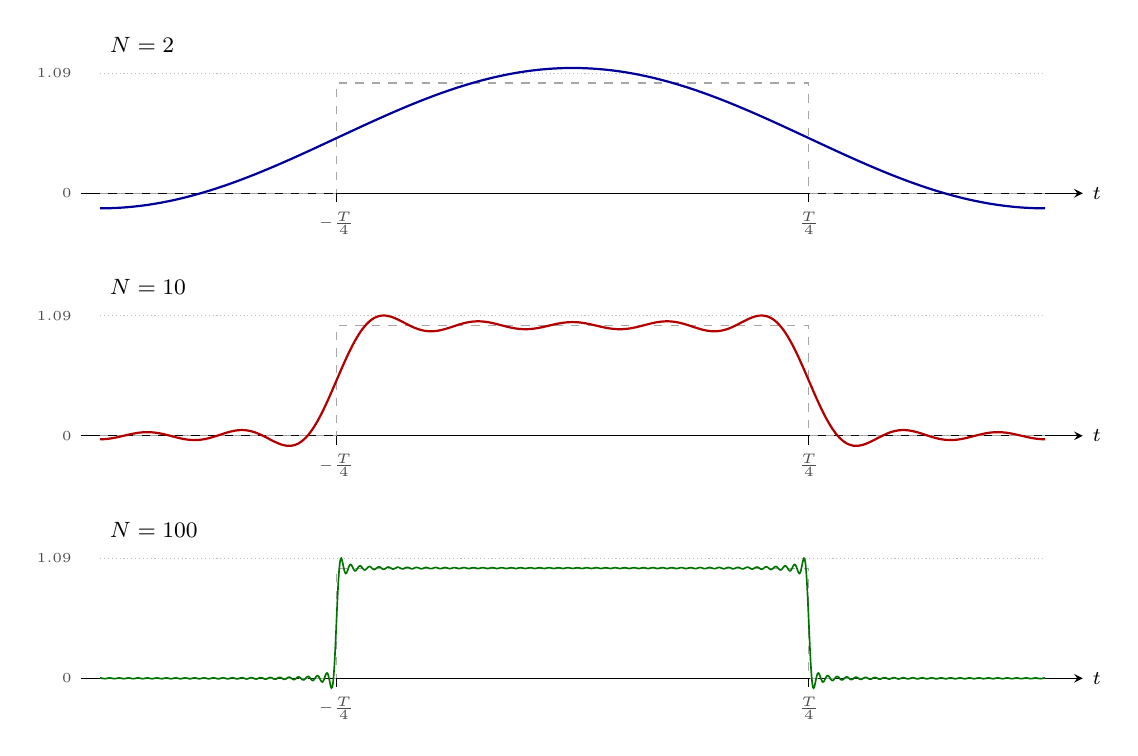
\begin{tikzpicture}[x=12cm,y=1.4cm]
  \foreach \N/\dy/\col in {2/0/blue!60!black,10/-2.2/red!70!black,100/-4.4/green!45!black}{
    \begin{scope}[shift={(0,\dy)}]
      \draw[->] (-0.52,0) -- (0.54,0) node[right,font=\scriptsize] {$t$};
      \draw[gray!70,dashed] (-0.5,0) -- (-0.25,0) -- (-0.25,1) -- (0.25,1) -- (0.25,0) -- (0.5,0);
      \draw[gray!50,densely dotted] (-0.5,1.09) -- (0.5,1.09);
      \foreach \p/\l in {-0.25/{-\frac T4},0.25/{\frac T4}}{\draw (\p,0) -- (\p,-0.08) node[anchor=north,font=\tiny,gray!60!black] {$\l$};}
      \node[anchor=east,font=\tiny,gray!60!black] at (-0.52,1.09) {$1.09$};
      \node[anchor=east,font=\tiny,gray!60!black] at (-0.52,0) {$0$};
      \node[font=\footnotesize,anchor=west] at (-0.5,1.35) {$N=\N$};
    \end{scope}}
  \draw[blue!60!black,thick] plot coordinates {(-0.5000,-0.1366) (-0.4950,-0.1363) (-0.4900,-0.1354) (-0.4850,-0.1338) (-0.4800,-0.1316) (-0.4750,-0.1288) (-0.4700,-0.1253) (-0.4650,-0.1213) (-0.4600,-0.1166) (-0.4550,-0.1113) (-0.4500,-0.1055) (-0.4450,-0.0990) (-0.4400,-0.0919) (-0.4350,-0.0843) (-0.4300,-0.0760) (-0.4250,-0.0672) (-0.4200,-0.0579) (-0.4150,-0.0480) (-0.4100,-0.0375) (-0.4050,-0.0265) (-0.4000,-0.0150) (-0.3950,-0.0030) (-0.3900,0.0095) (-0.3850,0.0225) (-0.3800,0.0359) (-0.3750,0.0498) (-0.3700,0.0642) (-0.3650,0.0790) (-0.3600,0.0942) (-0.3550,0.1098) (-0.3500,0.1258) (-0.3450,0.1422) (-0.3400,0.1589) (-0.3350,0.1759) (-0.3300,0.1933) (-0.3250,0.2110) (-0.3200,0.2289) (-0.3150,0.2472) (-0.3100,0.2656) (-0.3050,0.2844) (-0.3000,0.3033) (-0.2950,0.3224) (-0.2900,0.3417) (-0.2850,0.3611) (-0.2800,0.3807) (-0.2750,0.4004) (-0.2700,0.4202) (-0.2650,0.4401) (-0.2600,0.4600) (-0.2550,0.4800) (-0.2500,0.5000) (-0.2450,0.5200) (-0.2400,0.5400) (-0.2350,0.5599) (-0.2300,0.5798) (-0.2250,0.5996) (-0.2200,0.6193) (-0.2150,0.6389) (-0.2100,0.6583) (-0.2050,0.6776) (-0.2000,0.6967) (-0.1950,0.7156) (-0.1900,0.7344) (-0.1850,0.7528) (-0.1800,0.7711) (-0.1750,0.7890) (-0.1700,0.8067) (-0.1650,0.8241) (-0.1600,0.8411) (-0.1550,0.8578) (-0.1500,0.8742) (-0.1450,0.8902) (-0.1400,0.9058) (-0.1350,0.9210) (-0.1300,0.9358) (-0.1250,0.9502) (-0.1200,0.9641) (-0.1150,0.9775) (-0.1100,0.9905) (-0.1050,1.0030) (-0.1000,1.0150) (-0.0950,1.0265) (-0.0900,1.0375) (-0.0850,1.0480) (-0.0800,1.0579) (-0.0750,1.0672) (-0.0700,1.0760) (-0.0650,1.0843) (-0.0600,1.0919) (-0.0550,1.0990) (-0.0500,1.1055) (-0.0450,1.1113) (-0.0400,1.1166) (-0.0350,1.1213) (-0.0300,1.1253) (-0.0250,1.1288) (-0.0200,1.1316) (-0.0150,1.1338) (-0.0100,1.1354) (-0.0050,1.1363) (0.0000,1.1366) (0.0050,1.1363) (0.0100,1.1354) (0.0150,1.1338) (0.0200,1.1316) (0.0250,1.1288) (0.0300,1.1253) (0.0350,1.1213) (0.0400,1.1166) (0.0450,1.1113) (0.0500,1.1055) (0.0550,1.0990) (0.0600,1.0919) (0.0650,1.0843) (0.0700,1.0760) (0.0750,1.0672) (0.0800,1.0579) (0.0850,1.0480) (0.0900,1.0375) (0.0950,1.0265) (0.1000,1.0150) (0.1050,1.0030) (0.1100,0.9905) (0.1150,0.9775) (0.1200,0.9641) (0.1250,0.9502) (0.1300,0.9358) (0.1350,0.9210) (0.1400,0.9058) (0.1450,0.8902) (0.1500,0.8742) (0.1550,0.8578) (0.1600,0.8411) (0.1650,0.8241) (0.1700,0.8067) (0.1750,0.7890) (0.1800,0.7711) (0.1850,0.7528) (0.1900,0.7344) (0.1950,0.7156) (0.2000,0.6967) (0.2050,0.6776) (0.2100,0.6583) (0.2150,0.6389) (0.2200,0.6193) (0.2250,0.5996) (0.2300,0.5798) (0.2350,0.5599) (0.2400,0.5400) (0.2450,0.5200) (0.2500,0.5000) (0.2550,0.4800) (0.2600,0.4600) (0.2650,0.4401) (0.2700,0.4202) (0.2750,0.4004) (0.2800,0.3807) (0.2850,0.3611) (0.2900,0.3417) (0.2950,0.3224) (0.3000,0.3033) (0.3050,0.2844) (0.3100,0.2656) (0.3150,0.2472) (0.3200,0.2289) (0.3250,0.2110) (0.3300,0.1933) (0.3350,0.1759) (0.3400,0.1589) (0.3450,0.1422) (0.3500,0.1258) (0.3550,0.1098) (0.3600,0.0942) (0.3650,0.0790) (0.3700,0.0642) (0.3750,0.0498) (0.3800,0.0359) (0.3850,0.0225) (0.3900,0.0095) (0.3950,-0.0030) (0.4000,-0.0150) (0.4050,-0.0265) (0.4100,-0.0375) (0.4150,-0.0480) (0.4200,-0.0579) (0.4250,-0.0672) (0.4300,-0.0760) (0.4350,-0.0843) (0.4400,-0.0919) (0.4450,-0.0990) (0.4500,-0.1055) (0.4550,-0.1113) (0.4600,-0.1166) (0.4650,-0.1213) (0.4700,-0.1253) (0.4750,-0.1288) (0.4800,-0.1316) (0.4850,-0.1338) (0.4900,-0.1354) (0.4950,-0.1363) (0.5000,-0.1366)};
  \begin{scope}[shift={(0,-2.2)}]\draw[red!70!black,thick] plot coordinates {(-0.5000,-0.0315) (-0.4975,-0.0311) (-0.4950,-0.0300) (-0.4925,-0.0281) (-0.4900,-0.0254) (-0.4875,-0.0222) (-0.4850,-0.0184) (-0.4825,-0.0141) (-0.4800,-0.0094) (-0.4775,-0.0045) (-0.4750,0.0005) (-0.4725,0.0055) (-0.4700,0.0105) (-0.4675,0.0152) (-0.4650,0.0195) (-0.4625,0.0234) (-0.4600,0.0268) (-0.4575,0.0295) (-0.4550,0.0315) (-0.4525,0.0327) (-0.4500,0.0331) (-0.4475,0.0327) (-0.4450,0.0314) (-0.4425,0.0294) (-0.4400,0.0266) (-0.4375,0.0231) (-0.4350,0.0190) (-0.4325,0.0143) (-0.4300,0.0092) (-0.4275,0.0038) (-0.4250,-0.0017) (-0.4225,-0.0073) (-0.4200,-0.0128) (-0.4175,-0.0181) (-0.4150,-0.0231) (-0.4125,-0.0275) (-0.4100,-0.0313) (-0.4075,-0.0344) (-0.4050,-0.0367) (-0.4025,-0.0381) (-0.4000,-0.0386) (-0.3975,-0.0381) (-0.3950,-0.0367) (-0.3925,-0.0342) (-0.3900,-0.0309) (-0.3875,-0.0266) (-0.3850,-0.0216) (-0.3825,-0.0159) (-0.3800,-0.0096) (-0.3775,-0.0029) (-0.3750,0.0041) (-0.3725,0.0112) (-0.3700,0.0182) (-0.3675,0.0250) (-0.3650,0.0314) (-0.3625,0.0372) (-0.3600,0.0423) (-0.3575,0.0464) (-0.3550,0.0495) (-0.3525,0.0514) (-0.3500,0.0521) (-0.3475,0.0514) (-0.3450,0.0493) (-0.3425,0.0459) (-0.3400,0.0411) (-0.3375,0.0349) (-0.3350,0.0276) (-0.3325,0.0191) (-0.3300,0.0096) (-0.3275,-0.0006) (-0.3250,-0.0114) (-0.3225,-0.0225) (-0.3200,-0.0338) (-0.3175,-0.0448) (-0.3150,-0.0553) (-0.3125,-0.0650) (-0.3100,-0.0737) (-0.3075,-0.0809) (-0.3050,-0.0864) (-0.3025,-0.0899) (-0.3000,-0.0912) (-0.2975,-0.0899) (-0.2950,-0.0858) (-0.2925,-0.0787) (-0.2900,-0.0685) (-0.2875,-0.0550) (-0.2850,-0.0382) (-0.2825,-0.0179) (-0.2800,0.0057) (-0.2775,0.0328) (-0.2750,0.0631) (-0.2725,0.0967) (-0.2700,0.1332) (-0.2675,0.1725) (-0.2650,0.2143) (-0.2625,0.2583) (-0.2600,0.3043) (-0.2575,0.3518) (-0.2550,0.4005) (-0.2525,0.4501) (-0.2500,0.5000) (-0.2475,0.5499) (-0.2450,0.5995) (-0.2425,0.6482) (-0.2400,0.6957) (-0.2375,0.7417) (-0.2350,0.7857) (-0.2325,0.8275) (-0.2300,0.8668) (-0.2275,0.9033) (-0.2250,0.9369) (-0.2225,0.9672) (-0.2200,0.9943) (-0.2175,1.0179) (-0.2150,1.0382) (-0.2125,1.0550) (-0.2100,1.0685) (-0.2075,1.0787) (-0.2050,1.0858) (-0.2025,1.0899) (-0.2000,1.0912) (-0.1975,1.0899) (-0.1950,1.0864) (-0.1925,1.0809) (-0.1900,1.0737) (-0.1875,1.0650) (-0.1850,1.0553) (-0.1825,1.0448) (-0.1800,1.0338) (-0.1775,1.0225) (-0.1750,1.0114) (-0.1725,1.0006) (-0.1700,0.9904) (-0.1675,0.9809) (-0.1650,0.9724) (-0.1625,0.9651) (-0.1600,0.9589) (-0.1575,0.9541) (-0.1550,0.9507) (-0.1525,0.9486) (-0.1500,0.9479) (-0.1475,0.9486) (-0.1450,0.9505) (-0.1425,0.9536) (-0.1400,0.9577) (-0.1375,0.9628) (-0.1350,0.9686) (-0.1325,0.9750) (-0.1300,0.9818) (-0.1275,0.9888) (-0.1250,0.9959) (-0.1225,1.0029) (-0.1200,1.0096) (-0.1175,1.0159) (-0.1150,1.0216) (-0.1125,1.0266) (-0.1100,1.0309) (-0.1075,1.0342) (-0.1050,1.0367) (-0.1025,1.0381) (-0.1000,1.0386) (-0.0975,1.0381) (-0.0950,1.0367) (-0.0925,1.0344) (-0.0900,1.0313) (-0.0875,1.0275) (-0.0850,1.0231) (-0.0825,1.0181) (-0.0800,1.0128) (-0.0775,1.0073) (-0.0750,1.0017) (-0.0725,0.9962) (-0.0700,0.9908) (-0.0675,0.9857) (-0.0650,0.9810) (-0.0625,0.9769) (-0.0600,0.9734) (-0.0575,0.9706) (-0.0550,0.9686) (-0.0525,0.9673) (-0.0500,0.9669) (-0.0475,0.9673) (-0.0450,0.9685) (-0.0425,0.9705) (-0.0400,0.9732) (-0.0375,0.9766) (-0.0350,0.9805) (-0.0325,0.9848) (-0.0300,0.9895) (-0.0275,0.9945) (-0.0250,0.9995) (-0.0225,1.0045) (-0.0200,1.0094) (-0.0175,1.0141) (-0.0150,1.0184) (-0.0125,1.0222) (-0.0100,1.0254) (-0.0075,1.0281) (-0.0050,1.0300) (-0.0025,1.0311) (0.0000,1.0315) (0.0025,1.0311) (0.0050,1.0300) (0.0075,1.0281) (0.0100,1.0254) (0.0125,1.0222) (0.0150,1.0184) (0.0175,1.0141) (0.0200,1.0094) (0.0225,1.0045) (0.0250,0.9995) (0.0275,0.9945) (0.0300,0.9895) (0.0325,0.9848) (0.0350,0.9805) (0.0375,0.9766) (0.0400,0.9732) (0.0425,0.9705) (0.0450,0.9685) (0.0475,0.9673) (0.0500,0.9669) (0.0525,0.9673) (0.0550,0.9686) (0.0575,0.9706) (0.0600,0.9734) (0.0625,0.9769) (0.0650,0.9810) (0.0675,0.9857) (0.0700,0.9908) (0.0725,0.9962) (0.0750,1.0017) (0.0775,1.0073) (0.0800,1.0128) (0.0825,1.0181) (0.0850,1.0231) (0.0875,1.0275) (0.0900,1.0313) (0.0925,1.0344) (0.0950,1.0367) (0.0975,1.0381) (0.1000,1.0386) (0.1025,1.0381) (0.1050,1.0367) (0.1075,1.0342) (0.1100,1.0309) (0.1125,1.0266) (0.1150,1.0216) (0.1175,1.0159) (0.1200,1.0096) (0.1225,1.0029) (0.1250,0.9959) (0.1275,0.9888) (0.1300,0.9818) (0.1325,0.9750) (0.1350,0.9686) (0.1375,0.9628) (0.1400,0.9577) (0.1425,0.9536) (0.1450,0.9505) (0.1475,0.9486) (0.1500,0.9479) (0.1525,0.9486) (0.1550,0.9507) (0.1575,0.9541) (0.1600,0.9589) (0.1625,0.9651) (0.1650,0.9724) (0.1675,0.9809) (0.1700,0.9904) (0.1725,1.0006) (0.1750,1.0114) (0.1775,1.0225) (0.1800,1.0338) (0.1825,1.0448) (0.1850,1.0553) (0.1875,1.0650) (0.1900,1.0737) (0.1925,1.0809) (0.1950,1.0864) (0.1975,1.0899) (0.2000,1.0912) (0.2025,1.0899) (0.2050,1.0858) (0.2075,1.0787) (0.2100,1.0685) (0.2125,1.0550) (0.2150,1.0382) (0.2175,1.0179) (0.2200,0.9943) (0.2225,0.9672) (0.2250,0.9369) (0.2275,0.9033) (0.2300,0.8668) (0.2325,0.8275) (0.2350,0.7857) (0.2375,0.7417) (0.2400,0.6957) (0.2425,0.6482) (0.2450,0.5995) (0.2475,0.5499) (0.2500,0.5000) (0.2525,0.4501) (0.2550,0.4005) (0.2575,0.3518) (0.2600,0.3043) (0.2625,0.2583) (0.2650,0.2143) (0.2675,0.1725) (0.2700,0.1332) (0.2725,0.0967) (0.2750,0.0631) (0.2775,0.0328) (0.2800,0.0057) (0.2825,-0.0179) (0.2850,-0.0382) (0.2875,-0.0550) (0.2900,-0.0685) (0.2925,-0.0787) (0.2950,-0.0858) (0.2975,-0.0899) (0.3000,-0.0912) (0.3025,-0.0899) (0.3050,-0.0864) (0.3075,-0.0809) (0.3100,-0.0737) (0.3125,-0.0650) (0.3150,-0.0553) (0.3175,-0.0448) (0.3200,-0.0338) (0.3225,-0.0225) (0.3250,-0.0114) (0.3275,-0.0006) (0.3300,0.0096) (0.3325,0.0191) (0.3350,0.0276) (0.3375,0.0349) (0.3400,0.0411) (0.3425,0.0459) (0.3450,0.0493) (0.3475,0.0514) (0.3500,0.0521) (0.3525,0.0514) (0.3550,0.0495) (0.3575,0.0464) (0.3600,0.0423) (0.3625,0.0372) (0.3650,0.0314) (0.3675,0.0250) (0.3700,0.0182) (0.3725,0.0112) (0.3750,0.0041) (0.3775,-0.0029) (0.3800,-0.0096) (0.3825,-0.0159) (0.3850,-0.0216) (0.3875,-0.0266) (0.3900,-0.0309) (0.3925,-0.0342) (0.3950,-0.0367) (0.3975,-0.0381) (0.4000,-0.0386) (0.4025,-0.0381) (0.4050,-0.0367) (0.4075,-0.0344) (0.4100,-0.0313) (0.4125,-0.0275) (0.4150,-0.0231) (0.4175,-0.0181) (0.4200,-0.0128) (0.4225,-0.0073) (0.4250,-0.0017) (0.4275,0.0038) (0.4300,0.0092) (0.4325,0.0143) (0.4350,0.0190) (0.4375,0.0231) (0.4400,0.0266) (0.4425,0.0294) (0.4450,0.0314) (0.4475,0.0327) (0.4500,0.0331) (0.4525,0.0327) (0.4550,0.0315) (0.4575,0.0295) (0.4600,0.0268) (0.4625,0.0234) (0.4650,0.0195) (0.4675,0.0152) (0.4700,0.0105) (0.4725,0.0055) (0.4750,0.0005) (0.4775,-0.0045) (0.4800,-0.0094) (0.4825,-0.0141) (0.4850,-0.0184) (0.4875,-0.0222) (0.4900,-0.0254) (0.4925,-0.0281) (0.4950,-0.0300) (0.4975,-0.0311) (0.5000,-0.0315)};\end{scope}
  \begin{scope}[shift={(0,-4.4)}]\draw[green!45!black,line width=0.6pt] plot coordinates {(-0.5000,0.0032) (-0.4992,0.0028) (-0.4984,0.0017) (-0.4976,0.0002) (-0.4968,-0.0014) (-0.4960,-0.0026) (-0.4952,-0.0032) (-0.4944,-0.0030) (-0.4936,-0.0020) (-0.4928,-0.0006) (-0.4920,0.0010) (-0.4912,0.0023) (-0.4904,0.0031) (-0.4896,0.0031) (-0.4888,0.0023) (-0.4880,0.0010) (-0.4872,-0.0006) (-0.4864,-0.0020) (-0.4856,-0.0030) (-0.4848,-0.0032) (-0.4840,-0.0026) (-0.4832,-0.0014) (-0.4824,0.0002) (-0.4816,0.0017) (-0.4808,0.0028) (-0.4800,0.0032) (-0.4792,0.0028) (-0.4784,0.0017) (-0.4776,0.0002) (-0.4768,-0.0014) (-0.4760,-0.0026) (-0.4752,-0.0032) (-0.4744,-0.0030) (-0.4736,-0.0021) (-0.4728,-0.0006) (-0.4720,0.0010) (-0.4712,0.0024) (-0.4704,0.0031) (-0.4696,0.0031) (-0.4688,0.0024) (-0.4680,0.0010) (-0.4672,-0.0006) (-0.4664,-0.0021) (-0.4656,-0.0030) (-0.4648,-0.0032) (-0.4640,-0.0026) (-0.4632,-0.0014) (-0.4624,0.0002) (-0.4616,0.0018) (-0.4608,0.0029) (-0.4600,0.0033) (-0.4592,0.0029) (-0.4584,0.0018) (-0.4576,0.0002) (-0.4568,-0.0014) (-0.4560,-0.0027) (-0.4552,-0.0033) (-0.4544,-0.0031) (-0.4536,-0.0021) (-0.4528,-0.0006) (-0.4520,0.0010) (-0.4512,0.0024) (-0.4504,0.0032) (-0.4496,0.0032) (-0.4488,0.0024) (-0.4480,0.0010) (-0.4472,-0.0006) (-0.4464,-0.0022) (-0.4456,-0.0031) (-0.4448,-0.0034) (-0.4440,-0.0027) (-0.4432,-0.0014) (-0.4424,0.0002) (-0.4416,0.0018) (-0.4408,0.0030) (-0.4400,0.0034) (-0.4392,0.0030) (-0.4384,0.0018) (-0.4376,0.0002) (-0.4368,-0.0015) (-0.4360,-0.0028) (-0.4352,-0.0034) (-0.4344,-0.0032) (-0.4336,-0.0022) (-0.4328,-0.0006) (-0.4320,0.0011) (-0.4312,0.0026) (-0.4304,0.0034) (-0.4296,0.0034) (-0.4288,0.0026) (-0.4280,0.0011) (-0.4272,-0.0007) (-0.4264,-0.0023) (-0.4256,-0.0033) (-0.4248,-0.0035) (-0.4240,-0.0029) (-0.4232,-0.0015) (-0.4224,0.0002) (-0.4216,0.0020) (-0.4208,0.0032) (-0.4200,0.0036) (-0.4192,0.0032) (-0.4184,0.0019) (-0.4176,0.0002) (-0.4168,-0.0016) (-0.4160,-0.0030) (-0.4152,-0.0037) (-0.4144,-0.0034) (-0.4136,-0.0024) (-0.4128,-0.0007) (-0.4120,0.0012) (-0.4112,0.0028) (-0.4104,0.0037) (-0.4096,0.0037) (-0.4088,0.0027) (-0.4080,0.0012) (-0.4072,-0.0007) (-0.4064,-0.0025) (-0.4056,-0.0036) (-0.4048,-0.0038) (-0.4040,-0.0031) (-0.4032,-0.0016) (-0.4024,0.0003) (-0.4016,0.0021) (-0.4008,0.0034) (-0.4000,0.0039) (-0.3992,0.0034) (-0.3984,0.0021) (-0.3976,0.0002) (-0.3968,-0.0017) (-0.3960,-0.0033) (-0.3952,-0.0040) (-0.3944,-0.0037) (-0.3936,-0.0026) (-0.3928,-0.0007) (-0.3920,0.0013) (-0.3912,0.0030) (-0.3904,0.0040) (-0.3896,0.0040) (-0.3888,0.0030) (-0.3880,0.0013) (-0.3872,-0.0008) (-0.3864,-0.0027) (-0.3856,-0.0039) (-0.3848,-0.0042) (-0.3840,-0.0034) (-0.3832,-0.0018) (-0.3824,0.0003) (-0.3816,0.0024) (-0.3808,0.0038) (-0.3800,0.0044) (-0.3792,0.0038) (-0.3784,0.0023) (-0.3776,0.0002) (-0.3768,-0.0019) (-0.3760,-0.0036) (-0.3752,-0.0045) (-0.3744,-0.0042) (-0.3736,-0.0029) (-0.3728,-0.0008) (-0.3720,0.0015) (-0.3712,0.0034) (-0.3704,0.0045) (-0.3696,0.0045) (-0.3688,0.0034) (-0.3680,0.0014) (-0.3672,-0.0009) (-0.3664,-0.0031) (-0.3656,-0.0045) (-0.3648,-0.0048) (-0.3640,-0.0039) (-0.3632,-0.0020) (-0.3624,0.0004) (-0.3616,0.0027) (-0.3608,0.0044) (-0.3600,0.0050) (-0.3592,0.0044) (-0.3584,0.0027) (-0.3576,0.0003) (-0.3568,-0.0022) (-0.3560,-0.0042) (-0.3552,-0.0052) (-0.3544,-0.0048) (-0.3536,-0.0033) (-0.3528,-0.0009) (-0.3520,0.0017) (-0.3512,0.0040) (-0.3504,0.0052) (-0.3496,0.0052) (-0.3488,0.0039) (-0.3480,0.0016) (-0.3472,-0.0011) (-0.3464,-0.0036) (-0.3456,-0.0053) (-0.3448,-0.0056) (-0.3440,-0.0046) (-0.3432,-0.0024) (-0.3424,0.0005) (-0.3416,0.0032) (-0.3408,0.0052) (-0.3400,0.0059) (-0.3392,0.0052) (-0.3384,0.0032) (-0.3376,0.0003) (-0.3368,-0.0027) (-0.3360,-0.0051) (-0.3352,-0.0062) (-0.3344,-0.0058) (-0.3336,-0.0040) (-0.3328,-0.0011) (-0.3320,0.0021) (-0.3312,0.0048) (-0.3304,0.0064) (-0.3296,0.0064) (-0.3288,0.0048) (-0.3280,0.0020) (-0.3272,-0.0014) (-0.3264,-0.0045) (-0.3256,-0.0065) (-0.3248,-0.0069) (-0.3240,-0.0057) (-0.3232,-0.0029) (-0.3224,0.0006) (-0.3216,0.0040) (-0.3208,0.0066) (-0.3200,0.0075) (-0.3192,0.0065) (-0.3184,0.0039) (-0.3176,0.0003) (-0.3168,-0.0035) (-0.3160,-0.0065) (-0.3152,-0.0079) (-0.3144,-0.0074) (-0.3136,-0.0051) (-0.3128,-0.0014) (-0.3120,0.0028) (-0.3112,0.0063) (-0.3104,0.0084) (-0.3096,0.0084) (-0.3088,0.0063) (-0.3080,0.0025) (-0.3072,-0.0019) (-0.3064,-0.0060) (-0.3056,-0.0087) (-0.3048,-0.0093) (-0.3040,-0.0076) (-0.3032,-0.0039) (-0.3024,0.0009) (-0.3016,0.0056) (-0.3008,0.0090) (-0.3000,0.0103) (-0.2992,0.0090) (-0.2984,0.0054) (-0.2976,0.0003) (-0.2968,-0.0050) (-0.2960,-0.0092) (-0.2952,-0.0113) (-0.2944,-0.0106) (-0.2936,-0.0072) (-0.2928,-0.0018) (-0.2920,0.0042) (-0.2912,0.0094) (-0.2904,0.0124) (-0.2896,0.0124) (-0.2888,0.0092) (-0.2880,0.0036) (-0.2872,-0.0031) (-0.2864,-0.0094) (-0.2856,-0.0135) (-0.2848,-0.0144) (-0.2840,-0.0117) (-0.2832,-0.0059) (-0.2824,0.0017) (-0.2816,0.0093) (-0.2808,0.0148) (-0.2800,0.0169) (-0.2792,0.0148) (-0.2784,0.0087) (-0.2776,0.0001) (-0.2768,-0.0090) (-0.2760,-0.0164) (-0.2752,-0.0200) (-0.2744,-0.0187) (-0.2736,-0.0125) (-0.2728,-0.0027) (-0.2720,0.0086) (-0.2712,0.0185) (-0.2704,0.0243) (-0.2696,0.0243) (-0.2688,0.0179) (-0.2680,0.0063) (-0.2672,-0.0080) (-0.2664,-0.0216) (-0.2656,-0.0308) (-0.2648,-0.0329) (-0.2640,-0.0264) (-0.2632,-0.0121) (-0.2624,0.0073) (-0.2616,0.0273) (-0.2608,0.0427) (-0.2600,0.0486) (-0.2592,0.0420) (-0.2584,0.0223) (-0.2576,-0.0077) (-0.2568,-0.0421) (-0.2560,-0.0724) (-0.2552,-0.0887) (-0.2544,-0.0818) (-0.2536,-0.0442) (-0.2528,0.0278) (-0.2520,0.1335) (-0.2512,0.2675) (-0.2504,0.4203) (-0.2496,0.5797) (-0.2488,0.7325) (-0.2480,0.8665) (-0.2472,0.9722) (-0.2464,1.0442) (-0.2456,1.0818) (-0.2448,1.0887) (-0.2440,1.0724) (-0.2432,1.0421) (-0.2424,1.0077) (-0.2416,0.9777) (-0.2408,0.9580) (-0.2400,0.9514) (-0.2392,0.9573) (-0.2384,0.9727) (-0.2376,0.9927) (-0.2368,1.0121) (-0.2360,1.0264) (-0.2352,1.0329) (-0.2344,1.0308) (-0.2336,1.0216) (-0.2328,1.0080) (-0.2320,0.9937) (-0.2312,0.9821) (-0.2304,0.9757) (-0.2296,0.9757) (-0.2288,0.9815) (-0.2280,0.9914) (-0.2272,1.0027) (-0.2264,1.0125) (-0.2256,1.0187) (-0.2248,1.0200) (-0.2240,1.0164) (-0.2232,1.0090) (-0.2224,0.9999) (-0.2216,0.9913) (-0.2208,0.9852) (-0.2200,0.9831) (-0.2192,0.9852) (-0.2184,0.9907) (-0.2176,0.9983) (-0.2168,1.0059) (-0.2160,1.0117) (-0.2152,1.0144) (-0.2144,1.0135) (-0.2136,1.0094) (-0.2128,1.0031) (-0.2120,0.9964) (-0.2112,0.9908) (-0.2104,0.9876) (-0.2096,0.9876) (-0.2088,0.9906) (-0.2080,0.9958) (-0.2072,1.0018) (-0.2064,1.0072) (-0.2056,1.0106) (-0.2048,1.0113) (-0.2040,1.0092) (-0.2032,1.0050) (-0.2024,0.9997) (-0.2016,0.9946) (-0.2008,0.9910) (-0.2000,0.9897) (-0.1992,0.9910) (-0.1984,0.9944) (-0.1976,0.9991) (-0.1968,1.0039) (-0.1960,1.0076) (-0.1952,1.0093) (-0.1944,1.0087) (-0.1936,1.0060) (-0.1928,1.0019) (-0.1920,0.9975) (-0.1912,0.9937) (-0.1904,0.9916) (-0.1896,0.9916) (-0.1888,0.9937) (-0.1880,0.9972) (-0.1872,1.0014) (-0.1864,1.0051) (-0.1856,1.0074) (-0.1848,1.0079) (-0.1840,1.0065) (-0.1832,1.0035) (-0.1824,0.9997) (-0.1816,0.9961) (-0.1808,0.9935) (-0.1800,0.9925) (-0.1792,0.9934) (-0.1784,0.9960) (-0.1776,0.9994) (-0.1768,1.0029) (-0.1760,1.0057) (-0.1752,1.0069) (-0.1744,1.0065) (-0.1736,1.0045) (-0.1728,1.0014) (-0.1720,0.9980) (-0.1712,0.9952) (-0.1704,0.9936) (-0.1696,0.9936) (-0.1688,0.9952) (-0.1680,0.9979) (-0.1672,1.0011) (-0.1664,1.0040) (-0.1656,1.0058) (-0.1648,1.0062) (-0.1640,1.0051) (-0.1632,1.0027) (-0.1624,0.9997) (-0.1616,0.9968) (-0.1608,0.9948) (-0.1600,0.9941) (-0.1592,0.9948) (-0.1584,0.9968) (-0.1576,0.9995) (-0.1568,1.0024) (-0.1560,1.0046) (-0.1552,1.0056) (-0.1544,1.0053) (-0.1536,1.0036) (-0.1528,1.0011) (-0.1520,0.9984) (-0.1512,0.9961) (-0.1504,0.9948) (-0.1496,0.9948) (-0.1488,0.9960) (-0.1480,0.9983) (-0.1472,1.0009) (-0.1464,1.0033) (-0.1456,1.0048) (-0.1448,1.0052) (-0.1440,1.0042) (-0.1432,1.0022) (-0.1424,0.9997) (-0.1416,0.9973) (-0.1408,0.9956) (-0.1400,0.9950) (-0.1392,0.9956) (-0.1384,0.9973) (-0.1376,0.9996) (-0.1368,1.0020) (-0.1360,1.0039) (-0.1352,1.0048) (-0.1344,1.0045) (-0.1336,1.0031) (-0.1328,1.0009) (-0.1320,0.9986) (-0.1312,0.9966) (-0.1304,0.9955) (-0.1296,0.9955) (-0.1288,0.9966) (-0.1280,0.9985) (-0.1272,1.0008) (-0.1264,1.0029) (-0.1256,1.0042) (-0.1248,1.0045) (-0.1240,1.0036) (-0.1232,1.0019) (-0.1224,0.9998) (-0.1216,0.9977) (-0.1208,0.9962) (-0.1200,0.9956) (-0.1192,0.9962) (-0.1184,0.9976) (-0.1176,0.9997) (-0.1168,1.0018) (-0.1160,1.0034) (-0.1152,1.0042) (-0.1144,1.0039) (-0.1136,1.0027) (-0.1128,1.0008) (-0.1120,0.9987) (-0.1112,0.9970) (-0.1104,0.9960) (-0.1096,0.9960) (-0.1088,0.9970) (-0.1080,0.9987) (-0.1072,1.0007) (-0.1064,1.0026) (-0.1056,1.0037) (-0.1048,1.0040) (-0.1040,1.0033) (-0.1032,1.0017) (-0.1024,0.9998) (-0.1016,0.9979) (-0.1008,0.9966) (-0.1000,0.9961) (-0.0992,0.9966) (-0.0984,0.9979) (-0.0976,0.9997) (-0.0968,1.0016) (-0.0960,1.0031) (-0.0952,1.0038) (-0.0944,1.0036) (-0.0936,1.0025) (-0.0928,1.0007) (-0.0920,0.9988) (-0.0912,0.9973) (-0.0904,0.9963) (-0.0896,0.9963) (-0.0888,0.9972) (-0.0880,0.9988) (-0.0872,1.0007) (-0.0864,1.0024) (-0.0856,1.0034) (-0.0848,1.0037) (-0.0840,1.0030) (-0.0832,1.0016) (-0.0824,0.9998) (-0.0816,0.9981) (-0.0808,0.9968) (-0.0800,0.9964) (-0.0792,0.9968) (-0.0784,0.9980) (-0.0776,0.9998) (-0.0768,1.0015) (-0.0760,1.0029) (-0.0752,1.0035) (-0.0744,1.0033) (-0.0736,1.0023) (-0.0728,1.0007) (-0.0720,0.9989) (-0.0712,0.9974) (-0.0704,0.9966) (-0.0696,0.9966) (-0.0688,0.9974) (-0.0680,0.9989) (-0.0672,1.0006) (-0.0664,1.0022) (-0.0656,1.0032) (-0.0648,1.0034) (-0.0640,1.0028) (-0.0632,1.0015) (-0.0624,0.9998) (-0.0616,0.9982) (-0.0608,0.9970) (-0.0600,0.9966) (-0.0592,0.9970) (-0.0584,0.9982) (-0.0576,0.9998) (-0.0568,1.0014) (-0.0560,1.0027) (-0.0552,1.0034) (-0.0544,1.0031) (-0.0536,1.0022) (-0.0528,1.0006) (-0.0520,0.9990) (-0.0512,0.9976) (-0.0504,0.9968) (-0.0496,0.9968) (-0.0488,0.9976) (-0.0480,0.9990) (-0.0472,1.0006) (-0.0464,1.0021) (-0.0456,1.0031) (-0.0448,1.0033) (-0.0440,1.0027) (-0.0432,1.0014) (-0.0424,0.9998) (-0.0416,0.9982) (-0.0408,0.9971) (-0.0400,0.9967) (-0.0392,0.9971) (-0.0384,0.9982) (-0.0376,0.9998) (-0.0368,1.0014) (-0.0360,1.0026) (-0.0352,1.0032) (-0.0344,1.0030) (-0.0336,1.0021) (-0.0328,1.0006) (-0.0320,0.9990) (-0.0312,0.9976) (-0.0304,0.9969) (-0.0296,0.9969) (-0.0288,0.9976) (-0.0280,0.9990) (-0.0272,1.0006) (-0.0264,1.0021) (-0.0256,1.0030) (-0.0248,1.0032) (-0.0240,1.0026) (-0.0232,1.0014) (-0.0224,0.9998) (-0.0216,0.9983) (-0.0208,0.9972) (-0.0200,0.9968) (-0.0192,0.9972) (-0.0184,0.9983) (-0.0176,0.9998) (-0.0168,1.0014) (-0.0160,1.0026) (-0.0152,1.0032) (-0.0144,1.0030) (-0.0136,1.0020) (-0.0128,1.0006) (-0.0120,0.9990) (-0.0112,0.9977) (-0.0104,0.9969) (-0.0096,0.9969) (-0.0088,0.9977) (-0.0080,0.9990) (-0.0072,1.0006) (-0.0064,1.0020) (-0.0056,1.0030) (-0.0048,1.0032) (-0.0040,1.0026) (-0.0032,1.0014) (-0.0024,0.9998) (-0.0016,0.9983) (-0.0008,0.9972) (0.0000,0.9968) (0.0008,0.9972) (0.0016,0.9983) (0.0024,0.9998) (0.0032,1.0014) (0.0040,1.0026) (0.0048,1.0032) (0.0056,1.0030) (0.0064,1.0020) (0.0072,1.0006) (0.0080,0.9990) (0.0088,0.9977) (0.0096,0.9969) (0.0104,0.9969) (0.0112,0.9977) (0.0120,0.9990) (0.0128,1.0006) (0.0136,1.0020) (0.0144,1.0030) (0.0152,1.0032) (0.0160,1.0026) (0.0168,1.0014) (0.0176,0.9998) (0.0184,0.9983) (0.0192,0.9972) (0.0200,0.9968) (0.0208,0.9972) (0.0216,0.9983) (0.0224,0.9998) (0.0232,1.0014) (0.0240,1.0026) (0.0248,1.0032) (0.0256,1.0030) (0.0264,1.0021) (0.0272,1.0006) (0.0280,0.9990) (0.0288,0.9976) (0.0296,0.9969) (0.0304,0.9969) (0.0312,0.9976) (0.0320,0.9990) (0.0328,1.0006) (0.0336,1.0021) (0.0344,1.0030) (0.0352,1.0032) (0.0360,1.0026) (0.0368,1.0014) (0.0376,0.9998) (0.0384,0.9982) (0.0392,0.9971) (0.0400,0.9967) (0.0408,0.9971) (0.0416,0.9982) (0.0424,0.9998) (0.0432,1.0014) (0.0440,1.0027) (0.0448,1.0033) (0.0456,1.0031) (0.0464,1.0021) (0.0472,1.0006) (0.0480,0.9990) (0.0488,0.9976) (0.0496,0.9968) (0.0504,0.9968) (0.0512,0.9976) (0.0520,0.9990) (0.0528,1.0006) (0.0536,1.0022) (0.0544,1.0031) (0.0552,1.0034) (0.0560,1.0027) (0.0568,1.0014) (0.0576,0.9998) (0.0584,0.9982) (0.0592,0.9970) (0.0600,0.9966) (0.0608,0.9970) (0.0616,0.9982) (0.0624,0.9998) (0.0632,1.0015) (0.0640,1.0028) (0.0648,1.0034) (0.0656,1.0032) (0.0664,1.0022) (0.0672,1.0006) (0.0680,0.9989) (0.0688,0.9974) (0.0696,0.9966) (0.0704,0.9966) (0.0712,0.9974) (0.0720,0.9989) (0.0728,1.0007) (0.0736,1.0023) (0.0744,1.0033) (0.0752,1.0035) (0.0760,1.0029) (0.0768,1.0015) (0.0776,0.9998) (0.0784,0.9980) (0.0792,0.9968) (0.0800,0.9964) (0.0808,0.9968) (0.0816,0.9981) (0.0824,0.9998) (0.0832,1.0016) (0.0840,1.0030) (0.0848,1.0037) (0.0856,1.0034) (0.0864,1.0024) (0.0872,1.0007) (0.0880,0.9988) (0.0888,0.9972) (0.0896,0.9963) (0.0904,0.9963) (0.0912,0.9973) (0.0920,0.9988) (0.0928,1.0007) (0.0936,1.0025) (0.0944,1.0036) (0.0952,1.0038) (0.0960,1.0031) (0.0968,1.0016) (0.0976,0.9997) (0.0984,0.9979) (0.0992,0.9966) (0.1000,0.9961) (0.1008,0.9966) (0.1016,0.9979) (0.1024,0.9998) (0.1032,1.0017) (0.1040,1.0033) (0.1048,1.0040) (0.1056,1.0037) (0.1064,1.0026) (0.1072,1.0007) (0.1080,0.9987) (0.1088,0.9970) (0.1096,0.9960) (0.1104,0.9960) (0.1112,0.9970) (0.1120,0.9987) (0.1128,1.0008) (0.1136,1.0027) (0.1144,1.0039) (0.1152,1.0042) (0.1160,1.0034) (0.1168,1.0018) (0.1176,0.9997) (0.1184,0.9976) (0.1192,0.9962) (0.1200,0.9956) (0.1208,0.9962) (0.1216,0.9977) (0.1224,0.9998) (0.1232,1.0019) (0.1240,1.0036) (0.1248,1.0045) (0.1256,1.0042) (0.1264,1.0029) (0.1272,1.0008) (0.1280,0.9985) (0.1288,0.9966) (0.1296,0.9955) (0.1304,0.9955) (0.1312,0.9966) (0.1320,0.9986) (0.1328,1.0009) (0.1336,1.0031) (0.1344,1.0045) (0.1352,1.0048) (0.1360,1.0039) (0.1368,1.0020) (0.1376,0.9996) (0.1384,0.9973) (0.1392,0.9956) (0.1400,0.9950) (0.1408,0.9956) (0.1416,0.9973) (0.1424,0.9997) (0.1432,1.0022) (0.1440,1.0042) (0.1448,1.0052) (0.1456,1.0048) (0.1464,1.0033) (0.1472,1.0009) (0.1480,0.9983) (0.1488,0.9960) (0.1496,0.9948) (0.1504,0.9948) (0.1512,0.9961) (0.1520,0.9984) (0.1528,1.0011) (0.1536,1.0036) (0.1544,1.0053) (0.1552,1.0056) (0.1560,1.0046) (0.1568,1.0024) (0.1576,0.9995) (0.1584,0.9968) (0.1592,0.9948) (0.1600,0.9941) (0.1608,0.9948) (0.1616,0.9968) (0.1624,0.9997) (0.1632,1.0027) (0.1640,1.0051) (0.1648,1.0062) (0.1656,1.0058) (0.1664,1.0040) (0.1672,1.0011) (0.1680,0.9979) (0.1688,0.9952) (0.1696,0.9936) (0.1704,0.9936) (0.1712,0.9952) (0.1720,0.9980) (0.1728,1.0014) (0.1736,1.0045) (0.1744,1.0065) (0.1752,1.0069) (0.1760,1.0057) (0.1768,1.0029) (0.1776,0.9994) (0.1784,0.9960) (0.1792,0.9934) (0.1800,0.9925) (0.1808,0.9935) (0.1816,0.9961) (0.1824,0.9997) (0.1832,1.0035) (0.1840,1.0065) (0.1848,1.0079) (0.1856,1.0074) (0.1864,1.0051) (0.1872,1.0014) (0.1880,0.9972) (0.1888,0.9937) (0.1896,0.9916) (0.1904,0.9916) (0.1912,0.9937) (0.1920,0.9975) (0.1928,1.0019) (0.1936,1.0060) (0.1944,1.0087) (0.1952,1.0093) (0.1960,1.0076) (0.1968,1.0039) (0.1976,0.9991) (0.1984,0.9944) (0.1992,0.9910) (0.2000,0.9897) (0.2008,0.9910) (0.2016,0.9946) (0.2024,0.9997) (0.2032,1.0050) (0.2040,1.0092) (0.2048,1.0113) (0.2056,1.0106) (0.2064,1.0072) (0.2072,1.0018) (0.2080,0.9958) (0.2088,0.9906) (0.2096,0.9876) (0.2104,0.9876) (0.2112,0.9908) (0.2120,0.9964) (0.2128,1.0031) (0.2136,1.0094) (0.2144,1.0135) (0.2152,1.0144) (0.2160,1.0117) (0.2168,1.0059) (0.2176,0.9983) (0.2184,0.9907) (0.2192,0.9852) (0.2200,0.9831) (0.2208,0.9852) (0.2216,0.9913) (0.2224,0.9999) (0.2232,1.0090) (0.2240,1.0164) (0.2248,1.0200) (0.2256,1.0187) (0.2264,1.0125) (0.2272,1.0027) (0.2280,0.9914) (0.2288,0.9815) (0.2296,0.9757) (0.2304,0.9757) (0.2312,0.9821) (0.2320,0.9937) (0.2328,1.0080) (0.2336,1.0216) (0.2344,1.0308) (0.2352,1.0329) (0.2360,1.0264) (0.2368,1.0121) (0.2376,0.9927) (0.2384,0.9727) (0.2392,0.9573) (0.2400,0.9514) (0.2408,0.9580) (0.2416,0.9777) (0.2424,1.0077) (0.2432,1.0421) (0.2440,1.0724) (0.2448,1.0887) (0.2456,1.0818) (0.2464,1.0442) (0.2472,0.9722) (0.2480,0.8665) (0.2488,0.7325) (0.2496,0.5797) (0.2504,0.4203) (0.2512,0.2675) (0.2520,0.1335) (0.2528,0.0278) (0.2536,-0.0442) (0.2544,-0.0818) (0.2552,-0.0887) (0.2560,-0.0724) (0.2568,-0.0421) (0.2576,-0.0077) (0.2584,0.0223) (0.2592,0.0420) (0.2600,0.0486) (0.2608,0.0427) (0.2616,0.0273) (0.2624,0.0073) (0.2632,-0.0121) (0.2640,-0.0264) (0.2648,-0.0329) (0.2656,-0.0308) (0.2664,-0.0216) (0.2672,-0.0080) (0.2680,0.0063) (0.2688,0.0179) (0.2696,0.0243) (0.2704,0.0243) (0.2712,0.0185) (0.2720,0.0086) (0.2728,-0.0027) (0.2736,-0.0125) (0.2744,-0.0187) (0.2752,-0.0200) (0.2760,-0.0164) (0.2768,-0.0090) (0.2776,0.0001) (0.2784,0.0087) (0.2792,0.0148) (0.2800,0.0169) (0.2808,0.0148) (0.2816,0.0093) (0.2824,0.0017) (0.2832,-0.0059) (0.2840,-0.0117) (0.2848,-0.0144) (0.2856,-0.0135) (0.2864,-0.0094) (0.2872,-0.0031) (0.2880,0.0036) (0.2888,0.0092) (0.2896,0.0124) (0.2904,0.0124) (0.2912,0.0094) (0.2920,0.0042) (0.2928,-0.0018) (0.2936,-0.0072) (0.2944,-0.0106) (0.2952,-0.0113) (0.2960,-0.0092) (0.2968,-0.0050) (0.2976,0.0003) (0.2984,0.0054) (0.2992,0.0090) (0.3000,0.0103) (0.3008,0.0090) (0.3016,0.0056) (0.3024,0.0009) (0.3032,-0.0039) (0.3040,-0.0076) (0.3048,-0.0093) (0.3056,-0.0087) (0.3064,-0.0060) (0.3072,-0.0019) (0.3080,0.0025) (0.3088,0.0063) (0.3096,0.0084) (0.3104,0.0084) (0.3112,0.0063) (0.3120,0.0028) (0.3128,-0.0014) (0.3136,-0.0051) (0.3144,-0.0074) (0.3152,-0.0079) (0.3160,-0.0065) (0.3168,-0.0035) (0.3176,0.0003) (0.3184,0.0039) (0.3192,0.0065) (0.3200,0.0075) (0.3208,0.0066) (0.3216,0.0040) (0.3224,0.0006) (0.3232,-0.0029) (0.3240,-0.0057) (0.3248,-0.0069) (0.3256,-0.0065) (0.3264,-0.0045) (0.3272,-0.0014) (0.3280,0.0020) (0.3288,0.0048) (0.3296,0.0064) (0.3304,0.0064) (0.3312,0.0048) (0.3320,0.0021) (0.3328,-0.0011) (0.3336,-0.0040) (0.3344,-0.0058) (0.3352,-0.0062) (0.3360,-0.0051) (0.3368,-0.0027) (0.3376,0.0003) (0.3384,0.0032) (0.3392,0.0052) (0.3400,0.0059) (0.3408,0.0052) (0.3416,0.0032) (0.3424,0.0005) (0.3432,-0.0024) (0.3440,-0.0046) (0.3448,-0.0056) (0.3456,-0.0053) (0.3464,-0.0036) (0.3472,-0.0011) (0.3480,0.0016) (0.3488,0.0039) (0.3496,0.0052) (0.3504,0.0052) (0.3512,0.0040) (0.3520,0.0017) (0.3528,-0.0009) (0.3536,-0.0033) (0.3544,-0.0048) (0.3552,-0.0052) (0.3560,-0.0042) (0.3568,-0.0022) (0.3576,0.0003) (0.3584,0.0027) (0.3592,0.0044) (0.3600,0.0050) (0.3608,0.0044) (0.3616,0.0027) (0.3624,0.0004) (0.3632,-0.0020) (0.3640,-0.0039) (0.3648,-0.0048) (0.3656,-0.0045) (0.3664,-0.0031) (0.3672,-0.0009) (0.3680,0.0014) (0.3688,0.0034) (0.3696,0.0045) (0.3704,0.0045) (0.3712,0.0034) (0.3720,0.0015) (0.3728,-0.0008) (0.3736,-0.0029) (0.3744,-0.0042) (0.3752,-0.0045) (0.3760,-0.0036) (0.3768,-0.0019) (0.3776,0.0002) (0.3784,0.0023) (0.3792,0.0038) (0.3800,0.0044) (0.3808,0.0038) (0.3816,0.0024) (0.3824,0.0003) (0.3832,-0.0018) (0.3840,-0.0034) (0.3848,-0.0042) (0.3856,-0.0039) (0.3864,-0.0027) (0.3872,-0.0008) (0.3880,0.0013) (0.3888,0.0030) (0.3896,0.0040) (0.3904,0.0040) (0.3912,0.0030) (0.3920,0.0013) (0.3928,-0.0007) (0.3936,-0.0026) (0.3944,-0.0037) (0.3952,-0.0040) (0.3960,-0.0033) (0.3968,-0.0017) (0.3976,0.0002) (0.3984,0.0021) (0.3992,0.0034) (0.4000,0.0039) (0.4008,0.0034) (0.4016,0.0021) (0.4024,0.0003) (0.4032,-0.0016) (0.4040,-0.0031) (0.4048,-0.0038) (0.4056,-0.0036) (0.4064,-0.0025) (0.4072,-0.0007) (0.4080,0.0012) (0.4088,0.0027) (0.4096,0.0037) (0.4104,0.0037) (0.4112,0.0028) (0.4120,0.0012) (0.4128,-0.0007) (0.4136,-0.0024) (0.4144,-0.0034) (0.4152,-0.0037) (0.4160,-0.0030) (0.4168,-0.0016) (0.4176,0.0002) (0.4184,0.0019) (0.4192,0.0032) (0.4200,0.0036) (0.4208,0.0032) (0.4216,0.0020) (0.4224,0.0002) (0.4232,-0.0015) (0.4240,-0.0029) (0.4248,-0.0035) (0.4256,-0.0033) (0.4264,-0.0023) (0.4272,-0.0007) (0.4280,0.0011) (0.4288,0.0026) (0.4296,0.0034) (0.4304,0.0034) (0.4312,0.0026) (0.4320,0.0011) (0.4328,-0.0006) (0.4336,-0.0022) (0.4344,-0.0032) (0.4352,-0.0034) (0.4360,-0.0028) (0.4368,-0.0015) (0.4376,0.0002) (0.4384,0.0018) (0.4392,0.0030) (0.4400,0.0034) (0.4408,0.0030) (0.4416,0.0018) (0.4424,0.0002) (0.4432,-0.0014) (0.4440,-0.0027) (0.4448,-0.0034) (0.4456,-0.0031) (0.4464,-0.0022) (0.4472,-0.0006) (0.4480,0.0010) (0.4488,0.0024) (0.4496,0.0032) (0.4504,0.0032) (0.4512,0.0024) (0.4520,0.0010) (0.4528,-0.0006) (0.4536,-0.0021) (0.4544,-0.0031) (0.4552,-0.0033) (0.4560,-0.0027) (0.4568,-0.0014) (0.4576,0.0002) (0.4584,0.0018) (0.4592,0.0029) (0.4600,0.0033) (0.4608,0.0029) (0.4616,0.0018) (0.4624,0.0002) (0.4632,-0.0014) (0.4640,-0.0026) (0.4648,-0.0032) (0.4656,-0.0030) (0.4664,-0.0021) (0.4672,-0.0006) (0.4680,0.0010) (0.4688,0.0024) (0.4696,0.0031) (0.4704,0.0031) (0.4712,0.0024) (0.4720,0.0010) (0.4728,-0.0006) (0.4736,-0.0021) (0.4744,-0.0030) (0.4752,-0.0032) (0.4760,-0.0026) (0.4768,-0.0014) (0.4776,0.0002) (0.4784,0.0017) (0.4792,0.0028) (0.4800,0.0032) (0.4808,0.0028) (0.4816,0.0017) (0.4824,0.0002) (0.4832,-0.0014) (0.4840,-0.0026) (0.4848,-0.0032) (0.4856,-0.0030) (0.4864,-0.0020) (0.4872,-0.0006) (0.4880,0.0010) (0.4888,0.0023) (0.4896,0.0031) (0.4904,0.0031) (0.4912,0.0023) (0.4920,0.0010) (0.4928,-0.0006) (0.4936,-0.0020) (0.4944,-0.0030) (0.4952,-0.0032) (0.4960,-0.0026) (0.4968,-0.0014) (0.4976,0.0002) (0.4984,0.0017) (0.4992,0.0028) (0.5000,0.0032)};\end{scope}
\end{tikzpicture}
\caption{占空比为 $\frac12$ 的方波（灰色虚线，周期 $T$）用前 $N$ 项逼近。$N=2$ 时只是粗略的形状；$N=10$、$N=100$ 越来越接近方波，但跳变处的过冲始终约为 $1.09$（点线），底部约 $-0.09$。}
\end{figure}

\point{原因。}余弦、正弦都是弯曲的信号。用弯曲的信号叠加去模拟直上直下的跳变，无论取多少项，都不可能把弯完全变直。

%==================================================================
\section{傅里叶级数的复数形式}\label{sec:complex}
\subsection{改用信号的记号}
推导时用的是热传导的记号：自变量 $x$（位置）、函数 $f$。按教材的习惯，把自变量换成 $t$、函数换成 $x$，即 $f(x)\to x(t)$，$\mathrm{d}x\to\mathrm{d}t$，所有公式照样成立。

\point{$x(t)$ 是周期信号。}$\cos(k\omega_0t)$ 的周期是 $\frac{2\pi}{k\omega_0}$，而 $T_0=\frac{2\pi}{\omega_0}$ 是它的 $k$ 倍，所以 $T_0$ 是所有谐波的公共周期，它们加在一起得到的 $x(t)$ 以 $T_0$ 为周期。这个假设是合理的：在热传导问题里，杆长就是 $T_0$，把杆上的温度一段一段重复下去，就得到以 $T_0$ 为周期的信号，叫做对 $x(t)$ 的周期延拓(periodic extension)。

\begin{figure}[H]
\centering
\begin{tikzpicture}[x=1.0cm,y=1.0cm]
  \taxes{-6.4}{6.6}{1.3}{-0.2}
  \foreach \s in {-6,-3,3}{\draw[sig,dashed,domain=0:3,samples=60] plot ({\x+\s},{0.6+0.3*cos(2*pi*\x/3 r)+0.15*sin(4*pi*\x/3 r)});}
  \draw[sig,domain=0:3,samples=60] plot (\x,{0.6+0.3*cos(2*pi*\x/3 r)+0.15*sin(4*pi*\x/3 r)});
  \xt{-6}{-2T_0}\xt{-3}{-T_0}\xt{3}{T_0}\xt{6}{2T_0}
  \draw[<->,gray] (0,1.15) -- (3,1.15) node[midway,above,font=\tiny] {杆长 $T_0$};
\end{tikzpicture}
\caption{实线是杆上 $[0,T_0]$ 的温度，虚线是把它周期延拓后的样子。}
\end{figure}

\point{积分可以取任意一个周期。}周期信号在任意一个长为 $T_0$ 的区间上积分都相同，所以 $\int_0^{T_0}$ 也可以写成 $\int_{-T_0/2}^{T_0/2}$，统一记作 $\int_{T_0}$。$x(t)\cos(k\omega_0t)$、$x(t)\sin(k\omega_0t)$ 也都以 $T_0$ 为周期，系数公式中的积分同样可以写成 $\int_{T_0}$。

\begin{remember}
\textbf{三角形式}（教材第 86 页式 (3-19)）：
\[
x(t)=B_0+\sum_{k=1}^{+\infty}B_k\cos(k\omega_0t)+\sum_{k=1}^{+\infty}C_k\sin(k\omega_0t),
\]
\[
B_0=\frac{1}{T_0}\int_{T_0}x(t)\,\mathrm{d}t,\qquad
B_k=\frac{2}{T_0}\int_{T_0}x(t)\cos(k\omega_0t)\,\mathrm{d}t,\qquad
C_k=\frac{2}{T_0}\int_{T_0}x(t)\sin(k\omega_0t)\,\mathrm{d}t .
\]
\textbf{复数形式}（教材第 86 页式 (3-16)(3-17)）：
\[
x(t)=\sum_{k=-\infty}^{+\infty}a_k\,e^{jk\omega_0t},\qquad
a_k=\frac{1}{T_0}\int_{T_0}x(t)\,e^{-jk\omega_0t}\,\mathrm{d}t,\qquad \omega_0=\frac{2\pi}{T_0}.
\]
\textbf{转换公式}（教材第 85 页式 (3-9)(3-10)）：
\[
\begin{cases}B_0=a_0,\\ B_k=a_k+a_{-k}\ (k\ne0),\\ C_k=j\,(a_k-a_{-k})\ (k\ne0);\end{cases}
\qquad\text{或}\qquad
\begin{cases}a_0=B_0,\\ a_k=\frac12(B_k-jC_k)\ (k\ge1),\\ a_{-k}=\frac12(B_k+jC_k)\ (k\ge1).\end{cases}
\]
\end{remember}

两种形式描述的是同一件事：$x(t)$ 由常数项、余弦项、正弦项叠加而成。复数形式只需记两个公式，三角形式要记四个，所以后面基本都用复数形式。复数形式的本质思想仍是三角形式。

\subsection{两种形式等价的证明}
从复数形式出发，把 $k$ 与 $-k$ 两项配对，用欧拉公式 $e^{\pm j\theta}=\cos\theta\pm j\sin\theta$ 展开：
\begin{align*}
x(t)&=\sum_{k=-\infty}^{+\infty}a_k\,e^{jk\omega_0t}
=a_0+\big(a_1e^{j\omega_0t}+a_{-1}e^{-j\omega_0t}\big)+\big(a_2e^{j2\omega_0t}+a_{-2}e^{-j2\omega_0t}\big)+\cdots,
\end{align*}
其中
\begin{align*}
a_1e^{j\omega_0t}+a_{-1}e^{-j\omega_0t}
&=a_1\cos(\omega_0t)+ja_1\sin(\omega_0t)+a_{-1}\cos(\omega_0t)-ja_{-1}\sin(\omega_0t)\\
&=(a_1+a_{-1})\cos(\omega_0t)+j(a_1-a_{-1})\sin(\omega_0t).
\end{align*}
与三角形式逐项对照：$a_0=B_0$，$a_1+a_{-1}=B_1$，$j(a_1-a_{-1})=C_1$。第 $k$ 对同理：
\[
a_k+a_{-k}=B_k,\qquad j(a_k-a_{-k})=C_k .
\]
反过来，把这两式看成关于 $a_k$、$a_{-k}$ 的方程组，解出 $a_k=\frac12(B_k-jC_k)$、$a_{-k}=\frac12(B_k+jC_k)$。

\point{直接验证 $a_k$ 的公式。}由欧拉公式，
\[
a_k=\frac{1}{T_0}\int_{T_0}x(t)\cos(k\omega_0t)\,\mathrm{d}t-j\,\frac{1}{T_0}\int_{T_0}x(t)\sin(k\omega_0t)\,\mathrm{d}t=\frac{B_k}{2}-j\frac{C_k}{2},
\]
与转换公式一致。

\point{复数的来历。}复数最早出现在解三次方程时：计算中途必须出现 $\sqrt{-1}$，最后又能消掉。高斯(Gauss)证明了 $n$ 次多项式方程恰有 $n$ 个复根（含重根），使多项式方程的理论完备，复数从此被广泛接受；后来物理学中做分解与合成，也发现用复数更方便。傅里叶本人很可能并没有用复数，他的理论就是把信号拆成常数项、余弦项、正弦项；复数形式是后人为方便而改写的。

%==================================================================
\section{例题：周期方波的傅里叶级数}\label{sec:ex}
\example{周期方波}{只有直流与余弦项}{教材第 87 页}
\textbf{题目}：$x(t)$ 以 $T$ 为周期，一个周期 $\big[-\frac T2,\frac T2\big]$ 内，$|t|<T_1$ 时为 $1$，其余为 $0$。求它的傅里叶级数。

\begin{figure}[H]
\centering
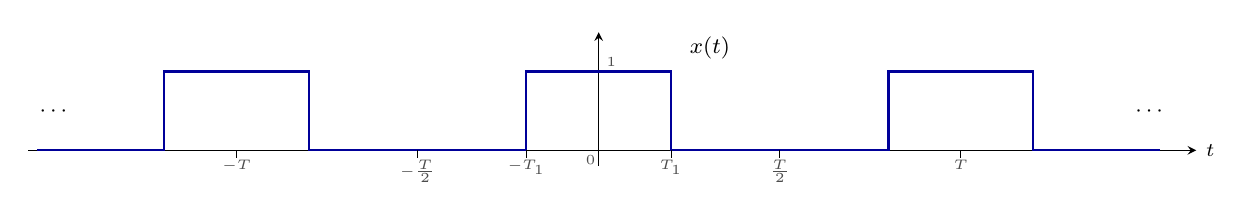
\begin{tikzpicture}[x=1.15cm,y=1.0cm]
  \taxes{-6.3}{6.6}{1.5}{-0.2}
  \foreach \c in {-4,0,4}{\draw[sig] ({\c-2},0) -- ({\c-0.8},0) -- ({\c-0.8},1) -- ({\c+0.8},1) -- ({\c+0.8},0) -- ({\c+2},0);}
  \draw[sig] (-6.2,0) -- (-6,0);\draw[sig] (6,0) -- (6.2,0);
  \node[font=\footnotesize] at (-6.0,0.5) {$\cdots$};\node[font=\footnotesize] at (6.1,0.5) {$\cdots$};
  \xt{-4}{-T}\xt{4}{T}\xt{-0.8}{-T_1}\xt{0.8}{T_1}\xt{-2}{-\frac T2}\xt{2}{\frac T2}
  \node[anchor=south west,font=\tiny,gray!60!black,inner sep=1pt] at (0.05,1.02) {$1$};
  \node[font=\footnotesize,anchor=west] at (0.9,1.3) {$x(t)$};
\end{tikzpicture}
\caption{周期为 $T$ 的方波：每个周期内 $|t|<T_1$ 处为 $1$。}
\end{figure}

注意：公式里的 $T_0$ 指一个周期的长度，这里一个周期是 $T$，所以 $T_0$ 换成 $T$，$\omega_0=\frac{2\pi}{T}$，即 $\omega_0T=2\pi$。不要死套公式，要理解了再代。积分取 $\big[-\frac T2,\frac T2\big]$ 这个周期最方便（取 $[0,T]$ 也一样，只是中间空跑一段）。

\subsection{解法一：三角形式}
\point{$B_0$。}在 $\big[-\frac T2,\frac T2\big]$ 内只有 $(-T_1,T_1)$ 上有值：
\[
B_0=\frac1T\int_{-T/2}^{T/2}x(t)\,\mathrm{d}t=\frac1T\int_{-T_1}^{T_1}\mathrm{d}t=\frac{2T_1}{T}.
\]
它就是 $x(t)$ 在一个周期内的平均值。

\point{$B_k$。}
\begin{align*}
B_k&=\frac2T\int_{-T_1}^{T_1}\cos(k\omega_0t)\,\mathrm{d}t=\frac2T\cdot\frac{1}{k\omega_0}\sin(k\omega_0t)\Big|_{-T_1}^{T_1}
=\frac2T\cdot\frac{1}{k\omega_0}\big[\sin(k\omega_0T_1)-\sin(-k\omega_0T_1)\big]\\
&=\frac{4}{kT\omega_0}\sin(k\omega_0T_1)=\frac{4}{2k\pi}\sin(k\omega_0T_1)=\frac{2}{k\pi}\sin\!\Big(\frac{2k\pi}{T}T_1\Big).
\end{align*}
第二行用了 $\sin$ 是奇函数（$-\sin(-\theta)=\sin\theta$）和 $\omega_0T=2\pi$。

\point{$C_k$。}
\[
C_k=\frac2T\int_{-T_1}^{T_1}\sin(k\omega_0t)\,\mathrm{d}t=0 :
\]
被积函数是奇函数，积分区间关于原点对称，正负两半相互抵消。

\point{结果。}
\[
x(t)=\frac{2T_1}{T}+\sum_{k=1}^{+\infty}\frac{2}{k\pi}\sin\!\Big(\frac{2k\pi}{T}T_1\Big)\cos(k\omega_0t).
\]

\subsection{从奇偶性一眼看出 \texorpdfstring{$C_k=0$}{Ck=0}}
$x(t)$ 是偶函数。三角形式中，$B_0+\sum B_k\cos(k\omega_0t)$ 全是偶函数，$\sum C_k\sin(k\omega_0t)$ 全是奇函数，所以三角形式本身就是把 $x(t)$ 分解成「偶函数 $+$ 奇函数」。由第一章，这种分解是唯一的：
\[
x(t)=\underbrace{\frac{x(t)+x(-t)}{2}}_{\text{偶部}}+\underbrace{\frac{x(t)-x(-t)}{2}}_{\text{奇部}} .
\]
$x(t)$ 是偶函数时奇部为 $0$，所以每个 $C_k$ 都为 $0$。

\begin{remember}
\begin{itemize}[nosep]
\item $x(t)$ 是偶函数 $\Rightarrow$ $C_k=0$，只需算 $B_0$、$B_k$；此时 $a_k=a_{-k}$。
\item $x(t)$ 是奇函数 $\Rightarrow$ $B_0=B_k=0$，只需算 $C_k$；此时由转换公式 $a_k=-\frac{j}{2}C_k$、$a_{-k}=\frac{j}{2}C_k$，即 $a_k=-a_{-k}$。
\end{itemize}
\end{remember}

\subsection{解法二：复数形式}
\point{$a_k$。}要熟记欧拉公式的两个推论
\[
\cos\alpha=\frac{e^{j\alpha}+e^{-j\alpha}}{2},\qquad \sin\alpha=\frac{e^{j\alpha}-e^{-j\alpha}}{2j}.
\]
\begin{align*}
a_k&=\frac1T\int_{-T_1}^{T_1}e^{-jk\omega_0t}\,\mathrm{d}t=\frac1T\cdot\frac{1}{-jk\omega_0}\,e^{-jk\omega_0t}\Big|_{-T_1}^{T_1}
=\frac1T\cdot\frac{1}{jk\omega_0}\big(e^{jk\omega_0T_1}-e^{-jk\omega_0T_1}\big)\\
&=\frac{2\sin(k\omega_0T_1)}{k\omega_0T}=\frac{\sin\!\big(\frac{2k\pi}{T}T_1\big)}{k\pi}.
\end{align*}
第二个等号把负号移进去、交换括号内两项的位置；第三个等号用了 $e^{j\alpha}-e^{-j\alpha}=2j\sin\alpha$。所以
\[
x(t)=\sum_{k=-\infty}^{+\infty}\frac{\sin\!\big(\frac{2k\pi}{T}T_1\big)}{k\pi}\,e^{jk\omega_0t}.
\]
做到这一步不算错，但还可以继续化简。

\point{$k=0$ 单独处理。}$k=0$ 时分子分母都为 $0$，要取极限。$k\to0$ 时 $\sin\theta\approx\theta$：
\[
a_0=\lim_{k\to0}\frac{\sin\!\big(\frac{2k\pi}{T}T_1\big)}{k\pi}=\frac{\frac{2k\pi}{T}T_1}{k\pi}=\frac{2T_1}{T},
\]
与 $B_0$ 相同。

\point{合并 $k$ 与 $-k$。}分子 $\sin\!\big(\frac{2k\pi}{T}T_1\big)$ 与分母 $k\pi$ 都是 $k$ 的奇函数，相除是 $k$ 的偶函数，所以 $a_k=a_{-k}$（与 $x(t)$ 是偶函数一致）。于是
\[
a_ke^{jk\omega_0t}+a_{-k}e^{-jk\omega_0t}=a_k\big(e^{jk\omega_0t}+e^{-jk\omega_0t}\big)=2a_k\cos(k\omega_0t),
\]
\[
x(t)=\frac{2T_1}{T}+\sum_{k=1}^{+\infty}\frac{2}{k\pi}\sin\!\Big(\frac{2k\pi}{T}T_1\Big)\cos(k\omega_0t),
\]
与解法一完全相同，也可以对照转换公式 $B_k=a_k+a_{-k}=2a_k$。

\begin{remember}
两种解法化到最简，答案完全一样：它们描述的都是「$x(t)$ 由常数项、余弦项、正弦项叠加而成」。转换公式不必死记，理解了算法，计算中自然能推出来。
\begin{itemize}[nosep]
\item 复数形式只需记两个公式；练熟以后通常更快。
\item 复数形式的做题流程：用 $a_k$ 公式积分 $\to$ 单独算 $a_0$（取极限）$\to$ 看 $x(t)$ 的奇偶性 $\to$ 把 $a_k$ 与 $a_{-k}$ 合并成余弦或正弦。
\end{itemize}
\end{remember}

\end{document}
